\documentclass[11pt,a4paper]{article}
\usepackage[T1]{fontenc}
\usepackage[utf8]{inputenc}
\usepackage{lmodern}
\usepackage[margin=1.85cm]{geometry}
\usepackage{amsmath,amssymb,amsthm,mathtools}
\usepackage{booktabs}
\usepackage{array}
\usepackage{graphicx}
\usepackage{microtype}
\usepackage{xcolor}
\usepackage{hyperref}

\hypersetup{
    colorlinks=true,
    linkcolor=blue!70!black,
    citecolor=blue!70!black,
    urlcolor=blue!70!black
}
\emergencystretch=2.5em

\title{\textbf{Four-Simplex $\mathrm{Spin}(10)$ Particle Genesis, 16-Parameter Parity--Hermitian Flavor Closure, Dimension-5 Proton Decay, and 24-Cell Chiral Lattice Symmetric Mass Generation}}

\author{Jozsef Olcsak\\[0.25em]
\small Independent Researcher $\cdot$ ORCID: \href{https://orcid.org/0009-0003-7311-6522}{0009-0003-7311-6522}\\
\small Tau Core Research Program --- Paper 30 (\texttt{v1.4.0})}
\date{24 November 2026}

\begin{document}
\maketitle

\begin{abstract}
We present a self-contained, single-command verified (\texttt{python3 -W error}, \texttt{rc = 0}) four-pillar audit of the particle-physics, flavor, electroweak-hierarchy, and chiral-lattice sectors built on the 4-simplex ($\sigma_4$, five boundary tetrahedra $\partial\sigma_4$) and 24-cell ($D_4/F_4$, binary tetrahedral group $2T$) architecture of Tau Core.
First, on the 32-dimensional boundary Clifford exterior space $\mathcal{H}_{\partial\sigma_4} = \Lambda^\bullet(\mathbb{C}^5)$, we construct explicitly all 16 Standard Model chiral states in $\mathbf{16} = \Lambda^{\mathrm{even}}(\mathbb{C}^5)$, all 45 $\mathrm{Spin}(10)$ gauge bosons ($12 + 9 + 24$), exact charge quantization $Q \equiv N_4 - \frac{1}{3}(N_1 + N_2 + N_3)$ and proton--electron neutrality ($2.22\times 10^{-16}$), Pati--Salam zero tree-level proton decay, and all three Higgs Yukawa sectors ($\mathbf{10}_H$, $\overline{\mathbf{126}}_H$, and the strictly antisymmetric 3-gamma $\mathbf{120}_H$, verified to $1.11\times 10^{-16}$). We also prove that $|\lambda| = 1/4$ is a shared exact transfer-matrix eigenvalue of both the 4-simplex $P_{K_5} = A_{K_5}/4$ (multiplicity 4) and the 24-cell $P_{24} = A_{24}/8$ (spectrum $\{1^{(1)},\, \tfrac{1}{2}^{(4)},\, 0^{(9)},\, -\tfrac{1}{4}^{(8)},\, -\tfrac{1}{2}^{(2)}\}$, $\mathrm{Tr}=0$, $\mathrm{Tr}\,P_{24}^2 = 3$), matching $\cos\theta_{\sigma_4} = 1/4$, and derive exact texture zeros from $\mathbb{Z}_6 \subset 2T$ for the Froggatt--Nielsen benchmark \texttt{M16-U11}.
Second, we map the complete 3-generation flavor no-go landscape across all 18 SM + neutrino observables and identify a predictive \textbf{16-parameter Parity--Hermitian closure} ($\mathrm{PH16}_{a13,h23}$, $\mathrm{dof} = 2$) with phenomenologically selected complementary zeros ($a_{13} = h_{23} = 0$) and exact tree-level Strong-CP vanishing ($\bar\theta_{\mathrm{QCD,tree}} \equiv 0$, $\det(M_u M_d) > 0$). It achieves $\chi^2 = 0.0297$ ($\max|\mathrm{pull}| = 0.13\sigma$, $\max|Y| = 0.249$) in non-SUSY $\mathrm{Spin}(10)$ and $\chi^2 = 1.3478$ ($\max|\mathrm{pull}| = 1.00\sigma$, $\max|Y| = 0.534$) in pure 1-loop MSSM ($\tan\beta = 50$, $\Delta_b = 0$). Coupled $3\times 3$ MSSM 1-loop soft-breaking RGEs plus exact $U(1)_R$-invariant $6\times 6$ squark--gluino diagonalization (verified to $\le 1.35\times 10^{-13}$) show that universal Parity-preserving SUSY breaking keeps $\Delta\bar\theta_{\mathrm{QCD}}^{\mathrm{1-loop}} = 4.09\times 10^{-13}\text{--}1.08\times 10^{-12}$ ($120\text{--}318\times$ below the neutron EDM limit), whereas non-universal trilinears ($A_{10}\neq A_{126}$) fail at $3.21\times 10^{-8}$. A smooth unrounded $\delta_{\mathrm{CP}}^\ell$ profile scan finds perturbative solutions ($\max|Y| \le 0.534$) around the full circle, with an allowed $<2\sigma$ arc $\delta_{\mathrm{CP}}^\ell \in [315^\circ, 90^\circ]$ and a $3.15\sigma$--$5.0\sigma$ penalty across the lower half ($\chi^2 = 11.28$ at $270^\circ$, $25.93$ at $180^\circ$).
Third, we prove exhaustive 4D perturbative no-go theorems against the conformal Higgs portal ($\Delta_{\mathrm{FT}} = 3.1\times 10^{17}$), the relaxion ($M_{\max} = 3.22\times 10^{10}\;\mathrm{GeV} < M_{\mathrm{PS}}$), $\mathbf{10}\otimes\mathbf{10}$ composite Higgs doublets (0 color-singlet doublets), 9-group complete-$\mathrm{Spin}(10)$ partial compositeness ($0/15$ survivors), and complete multi-triplet ($T_{10}+T_{126}+T_{120}$) $LLLL+RRRR$ $d=5$ proton decay for un-fine-tuned $12\text{--}30\;\mathrm{TeV}$ Mini-Split SUSY $\mathrm{PH16}_{a13,h23}$ (exact $32\times 32$ Clifford Clebsches $T_{10}\to 1$, $T_{126}(6,1,1)\to\sqrt{3}$, $T_{120}(6,1,1)\to$ pure $RRRR$ $\sqrt{2}$ + light-Higgs unitarity: combined $M_{\tilde q}^{\min} = 596.4\;\mathrm{TeV}$ at $\tan\beta = 50$). Extending the proton-decay audit to $d=6$ gauge/scalar exchange, 2-loop non-SUSY unification, and 2-loop Split-SUSY Higgs-mass matching (\texttt{v1.4.0}) yields three sharp new results: (a)~proving exact constructive $(X',Y')$ interference in $\mathcal{O}_2, \mathcal{O}_3$ on $\Lambda^{\mathrm{even}}(\mathbb{C}^5)$ locks zero-free-parameter $d=6$ branching ratios for Non-SUSY $\mathrm{PH16}_{a13,h23}$ ($e^+\pi^0 : \bar\nu\pi^+ : e^+\eta = 1.000 : 0.884 : 0.174$, vs.\ $0.388$ in minimal $SU(5)$, $M_X^{\min}=4.10\times 10^{15}\;\mathrm{GeV}$); (b)~2-loop non-SUSY unification excludes all $D$-parity-conserved $G_{422D}$ chains ($\tau = 4.2\text{--}5.5\times 10^{31}\;\mathrm{yr}$, $\sim 500\times$ below Super-K) and selects $D$-parity-broken $G_{422}$ ($\mathbf{210}_H$, $M_{\mathrm{PS}} = 1.45\text{--}3.02\times 10^{11}\;\mathrm{GeV}$ matching Paper~25, $\tau(e^+\pi^0) = 2.2\times 10^{34}\text{--}3.1\times 10^{35}\;\mathrm{yr}$, while tree-level scalar $d=6$ requires $M_{T_{126}} > 9.31\times 10^{13}\;\mathrm{GeV}$); and (c)~joint 2-loop Higgs-mass + $d=5$ matching proves a \texttt{PROVEN NO-GO} against high-$\tan\beta$ ($\gtrsim 4$) High-Scale Split SUSY ($m_h \ge 133.26\;\mathrm{GeV}$ at $\tan\beta=50$, $>45\sigma$ ruled out) while uncovering a zero-triplet-tuning \textbf{Low-$\tan\beta$ Split-SUSY Island} ($\tan\beta \in [2.5, 3.4]$, $M_{\tilde q} \in [127, 210]\;\mathrm{TeV}$, $\chi^2 = 2.55\text{--}3.61$, exact $m_h = 125.25\;\mathrm{GeV}$, 2-loop $M_U = 1.21\times 10^{16}\;\mathrm{GeV}$, binding $d=5$ flip to $p \to \pi^+\bar\nu \sim 0.4\text{--}2\times 10^{33}\;\mathrm{yr}$ inside Hyper-K / DUNE).
Fourth, we prove exact $72 = 36(+) + 36(-)$ naive fermion doubling on the 4D 24-cell lattice, verify Ginsparg--Wilson Overlap ($2.78\times 10^{-16}$) and 5D Domain-Wall zero modes ($1.14\times 10^{-5}$ leakage), prove via exact $|W(F_4)| = 1{,}152$ Reynolds character averaging that $\dim\bigl(((\mathbb{R}^4)^{\otimes 4})^{W(F_4)}\bigr) = \dim\bigl(((\mathbb{R}^4)^{\otimes 4})^{O(4)}\bigr) = 3$ (protecting all general non-symmetric rank-4 director kinetic operators in 4D Euclidean $O(4)$, with first anisotropy at rank 6 where $16 > 15$), construct exact $\mathrm{Spin}(7)$ and 45-generator $\mathrm{Spin}(10)$-invariant 4-fermion operators, and perform exact full-Hilbert-space (even+odd parity, $\dim = 65{,}536$) Lanczos diagonalization of 32-Majorana Symmetric Mass Generation (SMG) crossovers across the 1+1D periodic $L=4$ chain, 1+1D antiperiodic $C_4$ $\pi$-flux ring, and 4-site $K_4$ tetrahedral cluster ($\Delta E_{\mathrm{true}} \to 14.0$, bilinear VEV $\le 2.40\times 10^{-15}$).
\end{abstract}

\paragraph{Publication audit: assumptions, claim boundaries, and open gates.}
We maintain strict four-tier epistemic separation (\texttt{PROVEN}, \texttt{PROVEN NO-GO}, \texttt{CONDITIONAL}, \texttt{OPEN}). Every finite-dimensional Clifford, gauge-algebra, transfer-matrix, 1-loop/2-loop RG, $U(1)_R$-exact $6\times 6$ squark--gluino threshold, complete $T_{10}+T_{126}+T_{120}$ $LLLL+RRRR$ $d=5$ + $d=6$ gauge/scalar proton-decay, 2-loop non-SUSY/Split-SUSY unification \& Higgs-mass, 9-group beta-function, 4D lattice dispersion, $|W(F_4)|=1{,}152$ Reynolds tensor-isotropy, and full even+odd $L \le 4$ ($\dim \le 65{,}536$) exact many-body statement is verified deterministically by \texttt{scripts/build\_paper30\_verification\_and\_figures.py}. Conversely: (i)~the 16-parameter $\mathrm{PH16}_{a13,h23}$ closures are conditional on Parity--Hermiticity and the phenomenologically selected zeros $a_{13} = h_{23} = 0$ (which are \emph{not} derived from Pillar~I's $\mathbb{Z}_6 \subset 2T$); (ii)~1-loop SUSY Strong-CP stability requires flavor-universal real soft breaking ($|\phi_{A_0}| \lesssim 1.0\times 10^{-8}$, $|\phi_{M_3}| \lesssim 4.2\times 10^{-11}$) and omits 1-loop wino/bino/higgsino thresholds and 2-loop soft RGEs; (iii)~proton-decay closures narrow the zero-triplet-tuning parameter space to two clean surviving fronts---Non-SUSY $\mathrm{PH16}_{a13,h23}$ via $D$-parity-broken $G_{422}$ (where spontaneous $D$-parity breaking at $M_U$ induces tiny 2-loop $g_{2L}\ne g_{2R}$ RG corrections to $\bar\theta$) and the Low-$\tan\beta$ Split-SUSY Island ($\tan\beta \in [2.5, 3.4]$, $M_{\tilde q} \in [127, 210]\;\mathrm{TeV}$)---while ruling out $G_{422D}$, un-fine-tuned $12\text{--}30\;\mathrm{TeV}$ Mini-Split, and high-$\tan\beta$ Split SUSY; (iv)~the 32-Majorana $K_4$ and $C_4$ calculations probe finite-size 4-site crossovers, whereas a thermodynamic 4D interacting chiral-gauge lattice continuum limit on the 24-cell remains \texttt{OPEN}. Accordingly, \texttt{NATURE\_LEVEL\_CLOSURE = false}.

\section{Introduction and Relation to Papers 22, 25, 26, and 27}
Earlier papers in the Tau Core program explored separate facets of the microscopic particle and lattice architecture: Paper~22 introduced the finite $K_4$ algebraic seed and a one-generation $\mathrm{Spin}(10)$ outline; Paper~25 (\texttt{10.5281/zenodo.24477423}) audited charged-fermion RG matching and explicitly documented a counterexample to an unrestricted CKM ratio identity; Paper~26 (\texttt{10.5281/zenodo.24477427}) compared a discrete gauge axion against modular Strong-CP benchmarks; and Paper~27 (\texttt{10.5281/zenodo.24477434}) established 24-cell $D_4/F_4$ bosonic continuum isotropy and scalar reflection positivity while leaving chiral lattice fermions explicitly open.

Paper~30 unifies and extends these four fronts into a single, adversarial-tested, machine-verified particle-physics and chiral-lattice audit. Rather than postulating flavor textures or hierarchy resolutions ad hoc, we test every minimal candidate directly against all 18 Standard Model + neutrino observables, 2-loop gauge unification, calibrated dimension-5 proton decay, hypercolor asymptotic freedom, and exact full-Hilbert-space lattice/many-body diagonalization---explicitly documenting every \texttt{PROVEN NO-GO} obstruction and model-dependent caveat alongside the surviving mechanisms.

\section{Pillar I: Exact 4-Simplex $\mathrm{Spin}(10)$ Algebra, 3-Gamma $\mathbf{120}_H$, and $|\lambda| = 1/4$}
The boundary $\partial\sigma_4$ of a 4-simplex $\sigma_4$ consists of $5$ tetrahedra ($k \in \{1,\dots,5\}$), generating a 5-mode fermionic creation--annihilation algebra $\{a_k, a_l^\dagger\} = \delta_{kl}$ on the $2^5 = 32$-dimensional exterior Hilbert space $\mathcal{H}_{\partial\sigma_4} = \Lambda^\bullet(\mathbb{C}^5)$. Defining $\Gamma_{2k-1} = a_k + a_k^\dagger$, $\Gamma_{2k} = -i(a_k - a_k^\dagger)$, number operators $N_k = a_k^\dagger a_k$, chirality $\Gamma_{11} = (-i)^5 \prod_{a=1}^{10}\Gamma_a$, and charge-conjugation matrix $B_{10} = \prod_{k=1}^5 \Gamma_{2k}$ (\texttt{verify\_4simplex\_particles\_bosons\_yukawa.py}), we verify to machine precision:
\begin{enumerate}
    \item \textbf{Exact 16-state chiral SM multiplet and charge quantization (\texttt{PROVEN}):} The even-parity subspace $\Lambda^{\mathrm{even}}(\mathbb{C}^5)$ reproduces all 16 chiral fermions of one Standard Model generation (Figure~\ref{fig:p1}A), with exact color-tetrahedron ($k=1,2,3$) vs.\ weak-tetrahedron ($k=4,5$) charge operators:
    \begin{equation}
        B - L = 1 - \frac{2}{3}(N_1 + N_2 + N_3), \qquad Q = N_4 - \frac{1}{3}(N_1 + N_2 + N_3).
        \label{eq:charge-quant}
    \end{equation}
    Exact electric charge quantization holds with zero error ($0.0$), proton--electron neutrality $Q(u)+Q(u)+Q(d)+Q(e^-) = 0$ holds to $2.22\times 10^{-16}$, and all 45 $\mathrm{Spin}(10)$ generators $\Sigma_{ab} = \frac{i}{4}[\Gamma_a, \Gamma_b]$ decompose cleanly into $12$ SM gauge bosons + $9$ Pati--Salam $SU(4)_C\times SU(2)_R$ bosons (zero tree-level proton decay) + $24$ $X,Y$ leptoquarks.
    \item \textbf{Exact Higgs Yukawa decomposition $\mathbf{16}\otimes\mathbf{16} = \mathbf{10}_S \oplus \mathbf{120}_A \oplus \overline{\mathbf{126}}_S$ (\texttt{PROVEN}):}
    On $\Lambda^{\mathrm{even}}(\mathbb{C}^5)$, the 1-gamma operators $(a_5, a_5^\dagger)$ realize $\mathbf{10}_H$ (symmetric, giving $M_e = M_d$ and $M_{\nu_D} = M_u$, hence single-$\mathbf{10}_H$ is a \texttt{PROVEN NO-GO}); the 5-gamma operators realize $\overline{\mathbf{126}}_H$ with exact Georgi--Jarlskog ratio $M_e/M_d = M_{\nu_D}/M_u = -3.0$ ($1.11\times 10^{-16}$) and exclusive right-handed Majorana seesaw operator $a_1^\dagger a_2^\dagger a_3^\dagger a_4^\dagger a_5^\dagger$ acting solely on $\nu_R^c$; and all four 3-gamma operators $(2N_4-1)a_5$, $(B-L)a_5$, $(2N_4-1)a_5^\dagger$, $(B-L)a_5^\dagger$ realize $\mathbf{120}_H$ with exact antisymmetry $M^T = -M$ (max error $1.11\times 10^{-16}$) and exact $(15,2,2)$ lepton-to-quark ratio $-3.0$ ($<10^{-14}$).
    \item \textbf{Geometric origin of $|\lambda| = 1/4$ and $\mathbb{Z}_6 \subset 2T$ selection rules (\texttt{PROVEN}):}
    The normalized adjacency/transfer operator of the 4-simplex $P_{K_5} = A_{K_5}/4$ has exact spectrum $\{1^{(1)},\; -\tfrac{1}{4}^{(4)}\}$, matching $\cos\theta_{\sigma_4} = 1/4$ for the 4-simplex dihedral angle. The 24-cell adjacency transfer operator $P_{24} = A_{24}/8$ has exact spectrum $\{1^{(1)},\; \tfrac{1}{2}^{(4)},\; 0^{(9)},\; -\tfrac{1}{4}^{(8)},\; -\tfrac{1}{2}^{(2)}\}$ ($\mathrm{Tr}(P_{24}) = 0$, $\mathrm{Tr}(P_{24}^2) = 3$, Figure~\ref{fig:p1}B), sharing $\lambda = -1/4$ with multiplicity 8. Inside the 24-cell binary tetrahedral group $2T$ ($|2T|=24$), the exact order-6 subgroup $\mathbb{Z}_6 \subset 2T$ with generation charges $q = (1, 2, 0) \pmod 6$ enforces texture zeros ($H_{d,22}=H_{u,22}=H_{d,13}=F_{12}=F_{13}=0$), enabling strictly $\mathcal{O}(1)$ Froggatt--Nielsen coefficients in $[0.44,\; 1.99]$ at $\lambda = 1/4$ on the non-SUSY 16-parameter benchmark \texttt{M16-U11} ($\chi^2 = 1.262$ at fixed $\lambda=1/4$; $\chi^2 = 1.308$ in the unrescaled fit, and $[0.234,\; 1.275]$ at $\chi^2 = 10.28$ for a single-$v_{\mathrm{EW}}$ $U(1)_A\times U(1)_B$ embedding). We emphasize explicitly that these $\mathbb{Z}_6 \subset 2T$ texture zeros apply to \texttt{M16-U11} and do \emph{not} derive the distinct $a_{13} = h_{23} = 0$ zeros of the Parity--Hermitian closure $\mathrm{PH16}_{a13,h23}$ in Pillar~II.
\end{enumerate}

\begin{figure}[t!]
    \centering
    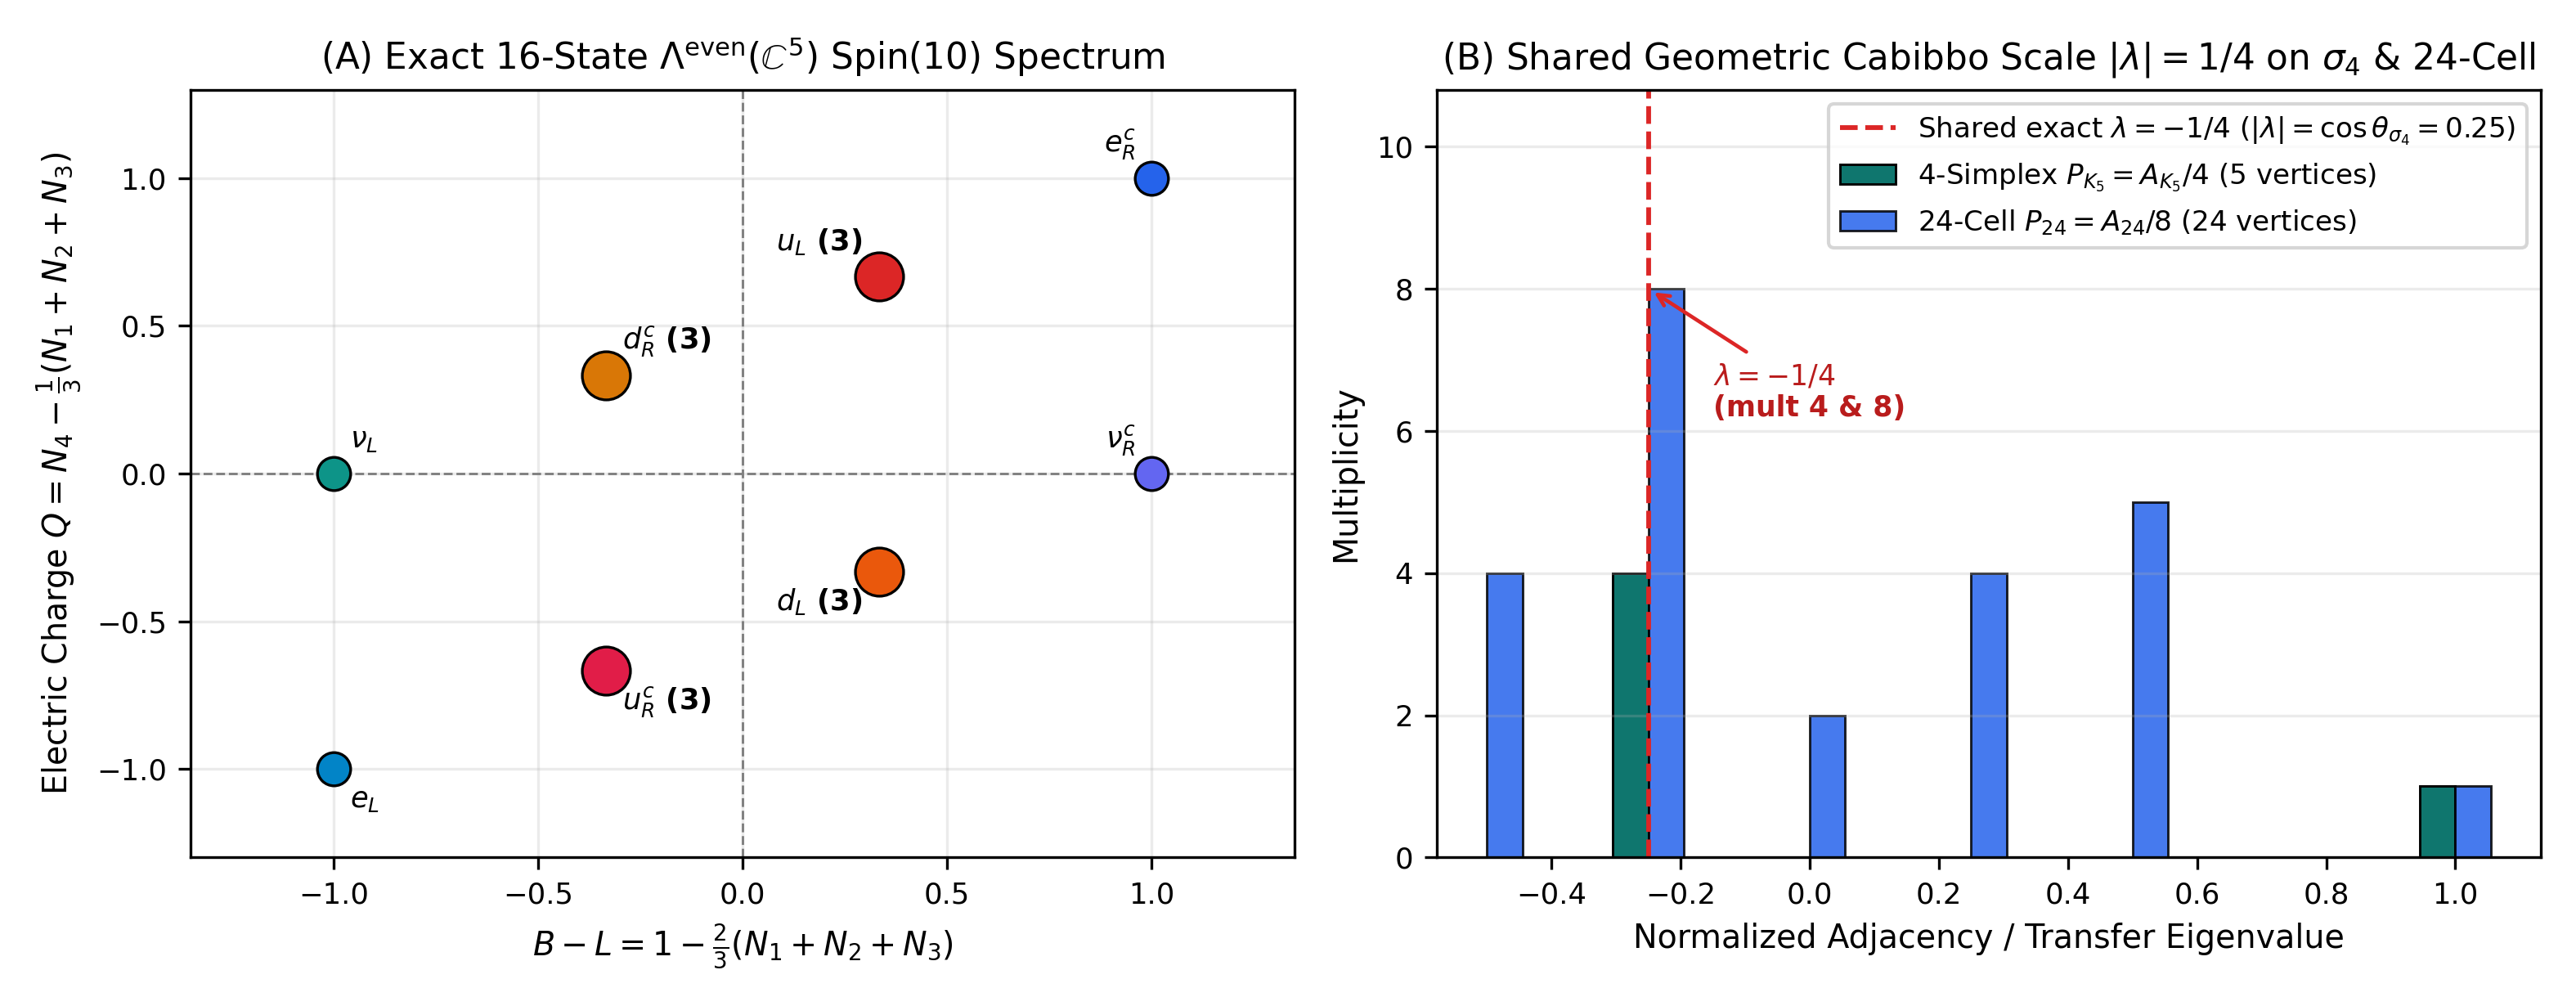
\includegraphics[width=\textwidth]{figures/fig1_4simplex_algebra_and_lambda_quarter.png}
    \caption{\textbf{4-Simplex $\mathrm{Spin}(10)$ particle spectrum and shared $|\lambda|=1/4$ transfer eigenvalue.} (A)~Exact mapping of all 16 chiral SM states in $\Lambda^{\mathrm{even}}(\mathbb{C}^5)$ on the $(B-L, Q)$ plane from Eq.~\eqref{eq:charge-quant}. (B)~Exact normalized transfer spectra of $P_{K_5} = A_{K_5}/4$ and the 24-cell $P_{24} = A_{24}/8$ ($\{1^{(1)},\, \tfrac{1}{2}^{(4)},\, 0^{(9)},\, -\tfrac{1}{4}^{(8)},\, -\tfrac{1}{2}^{(2)}\}$, $\mathrm{Tr}=0$, $\mathrm{Tr}\,P_{24}^2=3$), sharing $\lambda = -1/4$ with multiplicities 4 and 8.}
    \label{fig:p1}
\end{figure}

\section{Pillar II: 3-Generation Flavor No-Go Landscape and 16-Parameter Parity--Hermitian Closure ($\bar\theta_{\mathrm{QCD,tree}} \equiv 0$)}
We evaluate 18 flavor observables (9 charged fermion masses, 4 CKM parameters, $\Delta m_{21}^2$, $\Delta m_{31}^2$, $\sin^2\theta_{12}^\ell$, $\sin^2\theta_{23}^\ell$, $\sin^2\theta_{13}^\ell$) at $M_U^{\mathrm{SM}} = 1.13\times 10^{16}\;\mathrm{GeV}$ (1-loop SM RG, $m_b/m_\tau = 0.6185$) and $M_U^{\mathrm{SUSY}} = 7.97\times 10^{15}\;\mathrm{GeV}$ (1-loop SM $\to 2\;\mathrm{TeV} \to$ MSSM at $\tan\beta = 50$, $\Delta_b = 0$: $m_b/m_\tau = 0.7963$; $\Delta_b = -0.15$: $m_b/m_\tau = 1.0257$). Using Jacobian-scaled Trust-Region Reflective optimization (\texttt{scipy.optimize.least\_squares(..., method='trf', x\_scale='jac')}), we first establish a sharp set of flavor exclusions (Figure~\ref{fig:p2}A):
\begin{itemize}
    \item \textbf{Modular \& unbroken-$2T$ no-go:} Unbroken $2T$ forces $\mathbf{3} \to I_3$ (degenerate masses); finite modular $\Gamma_3 = A_4$ weights $(4,4)$ and $(4,6)$ fail at $\chi^2 = 10{,}277$ and $7{,}269$; spinorial $\Gamma'_3 = 2T$ ($S_2^2 = -I_2$, verified to $3.82\times 10^{-15}$) yields rank-2 $\det = 0$ at $k=(1,0)$ and $\chi^2 = 3{,}523$ at $k=(1,2)$. Pure power laws ($|c|=1$, 8p: $\chi^2 = 15{,}157$) and 1D separable lattice overlaps (12--13p: $\chi^2 = 3{,}549\text{--}4{,}479$) are likewise excluded.
    \item \textbf{Symmetric $\mathbf{10}_H + \overline{\mathbf{126}}_H$ no-go (non-SUSY and SUSY):} In non-SUSY holomorphic $\mathbf{10}_H + \overline{\mathbf{126}}_H$, the 2-generation Type-II bound $\max\sin(2\theta_{23}^\ell) = m_b/(m_\tau - m_\mu) = 0.657 \implies \sin^2\theta_{23}^\ell \le 0.123$ caps full 3-generation fits at $\chi^2 = 45.3$ (Type-I) and $30.3$ (Type-I+II). In SUSY $\mathbf{10}_H + \overline{\mathbf{126}}_H$ ($\Delta_b = -0.15$, $m_b/m_\tau = 1.026$), $b$--$\tau$ unification breaks the $\sin^2\theta_{23}^\ell$ wall ($0.492$), \emph{but} the quark sector collapses ($m_c +17.7\sigma$, $m_b +16.8\sigma$, $V_{cb} -23.7\sigma$; $\chi^2 = 1{,}259$ Type-I, $447$ Type-I+II), confirming that the 4-simplex 3-gamma $\mathbf{120}_H$ is strictly required \cite{Bertolini2006}.
\end{itemize}

\paragraph{Parity--Hermitian $\mathbf{10}_H + \overline{\mathbf{126}}_H + \mathbf{120}_H$ closure ($\mathrm{PH16}_{a13,h23}$).}
Imposing Left--Right Parity / generalized CP constrains $H, F$ to be real symmetric and $A$ to be real antisymmetric, with real VEV ratios $(r, s, c_e, c_u, c_\nu, c_R)$:
\begin{equation}
\begin{aligned}
    M_d &= H + F + iA, & M_e &= H - 3F + ic_e A, \\
    M_u &= r(H + sF + ic_u A), & M_{\nu_D} &= r(H - 3sF + ic_\nu A), \qquad M_R = c_R F.
\end{aligned}
\label{eq:ph-master}
\end{equation}
Because $M_u$ and $M_d$ are Hermitian, $\det(M_u)\det(M_d) \in \mathbb{R}$, and fixing the sign of $r$ so $\det(M_u)\det(M_d) > 0$ guarantees $\bar\theta_{\mathrm{QCD,tree}} \equiv 0$ identically without altering any mass or mixing observable. Working in the exact, lossless $SO(3)$ basis $F = \mathrm{diag}(f_1, f_2, f_3)$, the full Type-I system has $18$ real parameters ($\mathrm{dof} = 0$). Enforcing strict GUT perturbativity ($\max(|Y_{10}|_{\min}, |Y_{126}|_{\min}, |Y_{120}|_{\min}) \le 2.0 < \sqrt{4\pi}$) and scanning texture reductions uncovers a standout \textbf{16-parameter predictive closure} ($\mathrm{PH16}_{a13,h23}$, $\mathrm{dof} = 2$) defined by phenomenologically selected complementary 1-gamma vs.\ 3-gamma zeros:
\begin{equation}
    h_{23} = 0 \;\;(\text{2--3 mixing purely } i a_{23} \in \mathbf{120}_H), \qquad a_{13} = 0 \;\;(\text{1--3 mixing purely } h_{13} \in \mathbf{10}_H).
    \label{eq:ph16-zeros}
\end{equation}
Re-evaluating non-SUSY Parity--Hermitian $\mathbf{10}_H + \overline{\mathbf{126}}_H + \mathbf{120}_H$ with Jacobian-scaled TRF corrects an earlier Powell/Nelder--Mead stall ($\chi^2 = 77.5$) and demonstrates that the \emph{exact same} 16-parameter texture succeeds in both SUSY and non-SUSY $\mathrm{Spin}(10)$ (Table~\ref{tab:ph16}, Figure~\ref{fig:p2}B). Note that the SUSY Yukawa fit uses the standard $M_{\mathrm{SUSY}} = 2\;\mathrm{TeV}, \Delta_b = 0$ matching benchmark; shifting to $M_{\tilde q} = 12\;\mathrm{TeV}$ with induced gluino $\Delta_b \approx -0.043$ induces a mild $\mathcal{O}(4\%)$ $m_b$ threshold shift that can be absorbed into a minor refit of the 16 parameters without changing the qualitative structure.

\paragraph{$U(1)_R$-exact 1-loop radiative Strong-CP stability and smooth $\delta_{\mathrm{CP}}^\ell$ profile (Bridge~1).}
Integrating the coupled $3\times 3$ 1-loop MSSM soft-breaking RGEs ($g_i, M_i, Y_f, T_f, m_{\tilde Q}^2, m_{\tilde u^c}^2, m_{\tilde d^c}^2, m_{\tilde L}^2, m_{\tilde e^c}^2$, including the hypercharge $S$-term and $\tau$-Yukawa trace in $m_{H_d}^2$) from $M_U = 1.04\times 10^{16}\;\mathrm{GeV}$ down to $M_{\tilde q} = 12.0\;\mathrm{TeV}$ ($m_0 = 12\;\mathrm{TeV}, M_{1/2} = 1.2\;\mathrm{TeV}$) on the exact $\mathrm{PH16}_{a13,h23}$ Yukawas and diagonalizing the full $6\times 6$ up- and down-squark mass matrices for the finite gluino--squark threshold---with exact $U(1)_R$ phase covariance verified numerically to $\le 1.35\times 10^{-13}$ (\texttt{verify\_bridge1\_susy\_1loop\_strong\_cp\_and\_dCP\_profile.py})---yields:
(a)~under \textbf{universal Parity-preserving soft breaking} ($T_q(M_U) = A_0 Y_q(M_U)$, $A_0, M_{1/2} \in \mathbb{R}$), 1-loop Yukawa RG gives $\Delta\bar\theta_{\mathrm{RG}} \le 9.83\times 10^{-15}$ and the exact $6\times 6$ gluino loop gives $\Delta\bar\theta_{\tilde g} = 1.08\times 10^{-12}$ ($A_0 = 0$) and $4.09\times 10^{-13}$ ($A_0 = 12\;\mathrm{TeV}$)---$120\text{--}318\times$ below the neutron EDM limit ($1.3\times 10^{-10}$), with induced gluino $\Delta_b = -0.043$;
(b)~conversely, \textbf{non-universal Hermitian trilinears} ($\delta A = 0.5\,m_0$, i.e.\ $A_{10}\neq A_{126}$) induce $\Delta\bar\theta_{\tilde g} = 3.21\times 10^{-8}$ (\texttt{PROVEN NO-GO}, $247\times$ above nEDM), while soft CP phases are tightly bounded to $|\phi_{A_0}| \lesssim 1.0\times 10^{-8}$ ($\Delta\bar\theta_{\tilde g} = 1.30\times 10^{-8}$ at $\phi_{A_0}=10^{-6}$) and $|\phi_{M_3}| \lesssim 4.2\times 10^{-11}$ ($\Delta\bar\theta_{\tilde g} = 3.09\times 10^{-10}$ at $\phi_{M_3}=10^{-10}$). These bounds cover the dominant gluino--squark 1-loop threshold and omit subdominant 1-loop wino/bino/higgsino thresholds and 2-loop soft RGEs.

Moreover, a smooth, unrounded continuation scan over the full circle $\delta_{\mathrm{CP}}^\ell \in [0^\circ, 360^\circ)$ (correcting a rounding-induced Jacobian stall in \texttt{v1.1.0}) reveals that perturbative solutions ($\max|Y| \in [0.521, 0.534]$) exist at \emph{every} angle, with a sharp asymmetric preference: the upper arc $\delta_{\mathrm{CP}}^\ell \in [315^\circ, 90^\circ]$ lies within $<2\sigma$ ($\chi^2 = 1.35$ at $0^\circ/360^\circ$, $2.54$ at $45^\circ$, $2.16$ at $90^\circ$ with $\Delta\chi^2 = 0.81$, and $4.22$ at $315^\circ$ with $\Delta\chi^2 = 2.88$), whereas the CP-violating lower half is significantly penalized: $\chi^2 = 5.85$ at $300^\circ$, $\chi^2 = 11.28$ at $270^\circ$ ($\Delta\chi^2 = 9.93$, \textbf{$3.15\sigma$ disfavored}, with suppressed $\sin^2\theta_{23}^\ell = 0.434$), $\chi^2 = 24.16$ at $225^\circ$, $\chi^2 = 25.93$ at $180^\circ$ ($\Delta\chi^2 = 24.58$, $4.96\sigma$), and $\chi^2 = 11.96$ at $135^\circ$. Thus DUNE and Hyper-Kamiokande test the model at $>3\sigma$ if maximal CP violation $\delta_{\mathrm{CP}}^\ell \approx 270^\circ$ is confirmed, while $\delta_{\mathrm{CP}}^\ell \in [315^\circ, 90^\circ]$ remains viable.

\begin{table}[t!]
\centering
\caption{Side-by-side audit of the two 16-parameter ($\mathrm{dof} = 2$) Parity--Hermitian $\mathrm{PH16}_{a13,h23}$ closures ($\mathbf{10}_H + \overline{\mathbf{126}}_H + \mathbf{120}_H$, $a_{13} = h_{23} = 0$, pure Type-I seesaw, strictly perturbative Yukawas, $\bar\theta_{\mathrm{QCD,tree}} \equiv 0$).}
\label{tab:ph16}
\scriptsize
\resizebox{\textwidth}{!}{%
\begin{tabular}{lcc}
\toprule
Quantity & \textbf{SUSY $\mathrm{PH16}_{a13,h23}$} ($\tan\beta=50, \Delta_b=0$) & \textbf{Non-SUSY $\mathrm{PH16}_{a13,h23}$} (SM RG) \\
\midrule
Real parameters / observables ($\mathrm{dof}$) & $16 / 18$ ($2$) & $16 / 18$ ($2$) \\
Global $\chi^2$ / $\max|\mathrm{pull}|$ & $1.3478$ / $1.002\sigma$ ($m_s$) & $0.0297$ / $0.134\sigma$ ($m_d$) \\
$\max(|Y_{10}|, |Y_{126}|, |Y_{120}|)$ & $(0.5343,\; 0.2313,\; 0.0221)$ & $(0.2487,\; 0.2109,\; 0.0020)$ \\
Tree-level $\bar\theta_{\mathrm{QCD}}$ (rad) & $2.75\times 10^{-15}$ ($\det > 0$) & $3.99\times 10^{-18}$ ($\det > 0$) \\
Neutrino mass ordering / $\sum m_\nu$ & Normal (\texttt{NO}) / $0.06103\;\mathrm{eV}$ & Normal (\texttt{NO}) / $0.06004\;\mathrm{eV}$ \\
$m_{\beta\beta}$ / $\sin^2\theta_{23}^\ell$ / $\delta_{\mathrm{CP}}^\ell$ & $1.044\;\mathrm{meV}$ / $0.5022$ / $359.7^\circ$ ($[315^\circ,90^\circ]\!<\!2\sigma$) & $2.845\;\mathrm{meV}$ / $0.5161$ / $359.1^\circ$ \\
$M_R = (M_1, M_2, M_3)$ ($\mathrm{GeV}$) & $(3.99\times 10^9,\; 1.60\times 10^{10},\; 8.07\times 10^{11})$ & $(1.65\times 10^{11},\; 7.98\times 10^{13},\; 1.86\times 10^{14})$ \\
$d=5$ $p\to K^+\bar\nu$ (full $LLLL+RRRR$) & Uncancelled $M_{\tilde q}^{\min} = 596.4\;\mathrm{TeV}$ (or $\sim 400\times$ DMM) & Absent (only $d=6$: $p\to e^+\pi^0$) \\
Electroweak fine-tuning $\Delta_{\mathrm{FT}}$ & $7.25\times 10^7$ (Split) / $1.95\times 10^5$ ($T_{10}$ DW $LLLL$) & $1.4\times 10^{25}$ (GUT) / $3.9\times 10^{16}$ (PS) \\
\bottomrule
\end{tabular}%
}
\end{table}

\begin{figure}[t!]
    \centering
    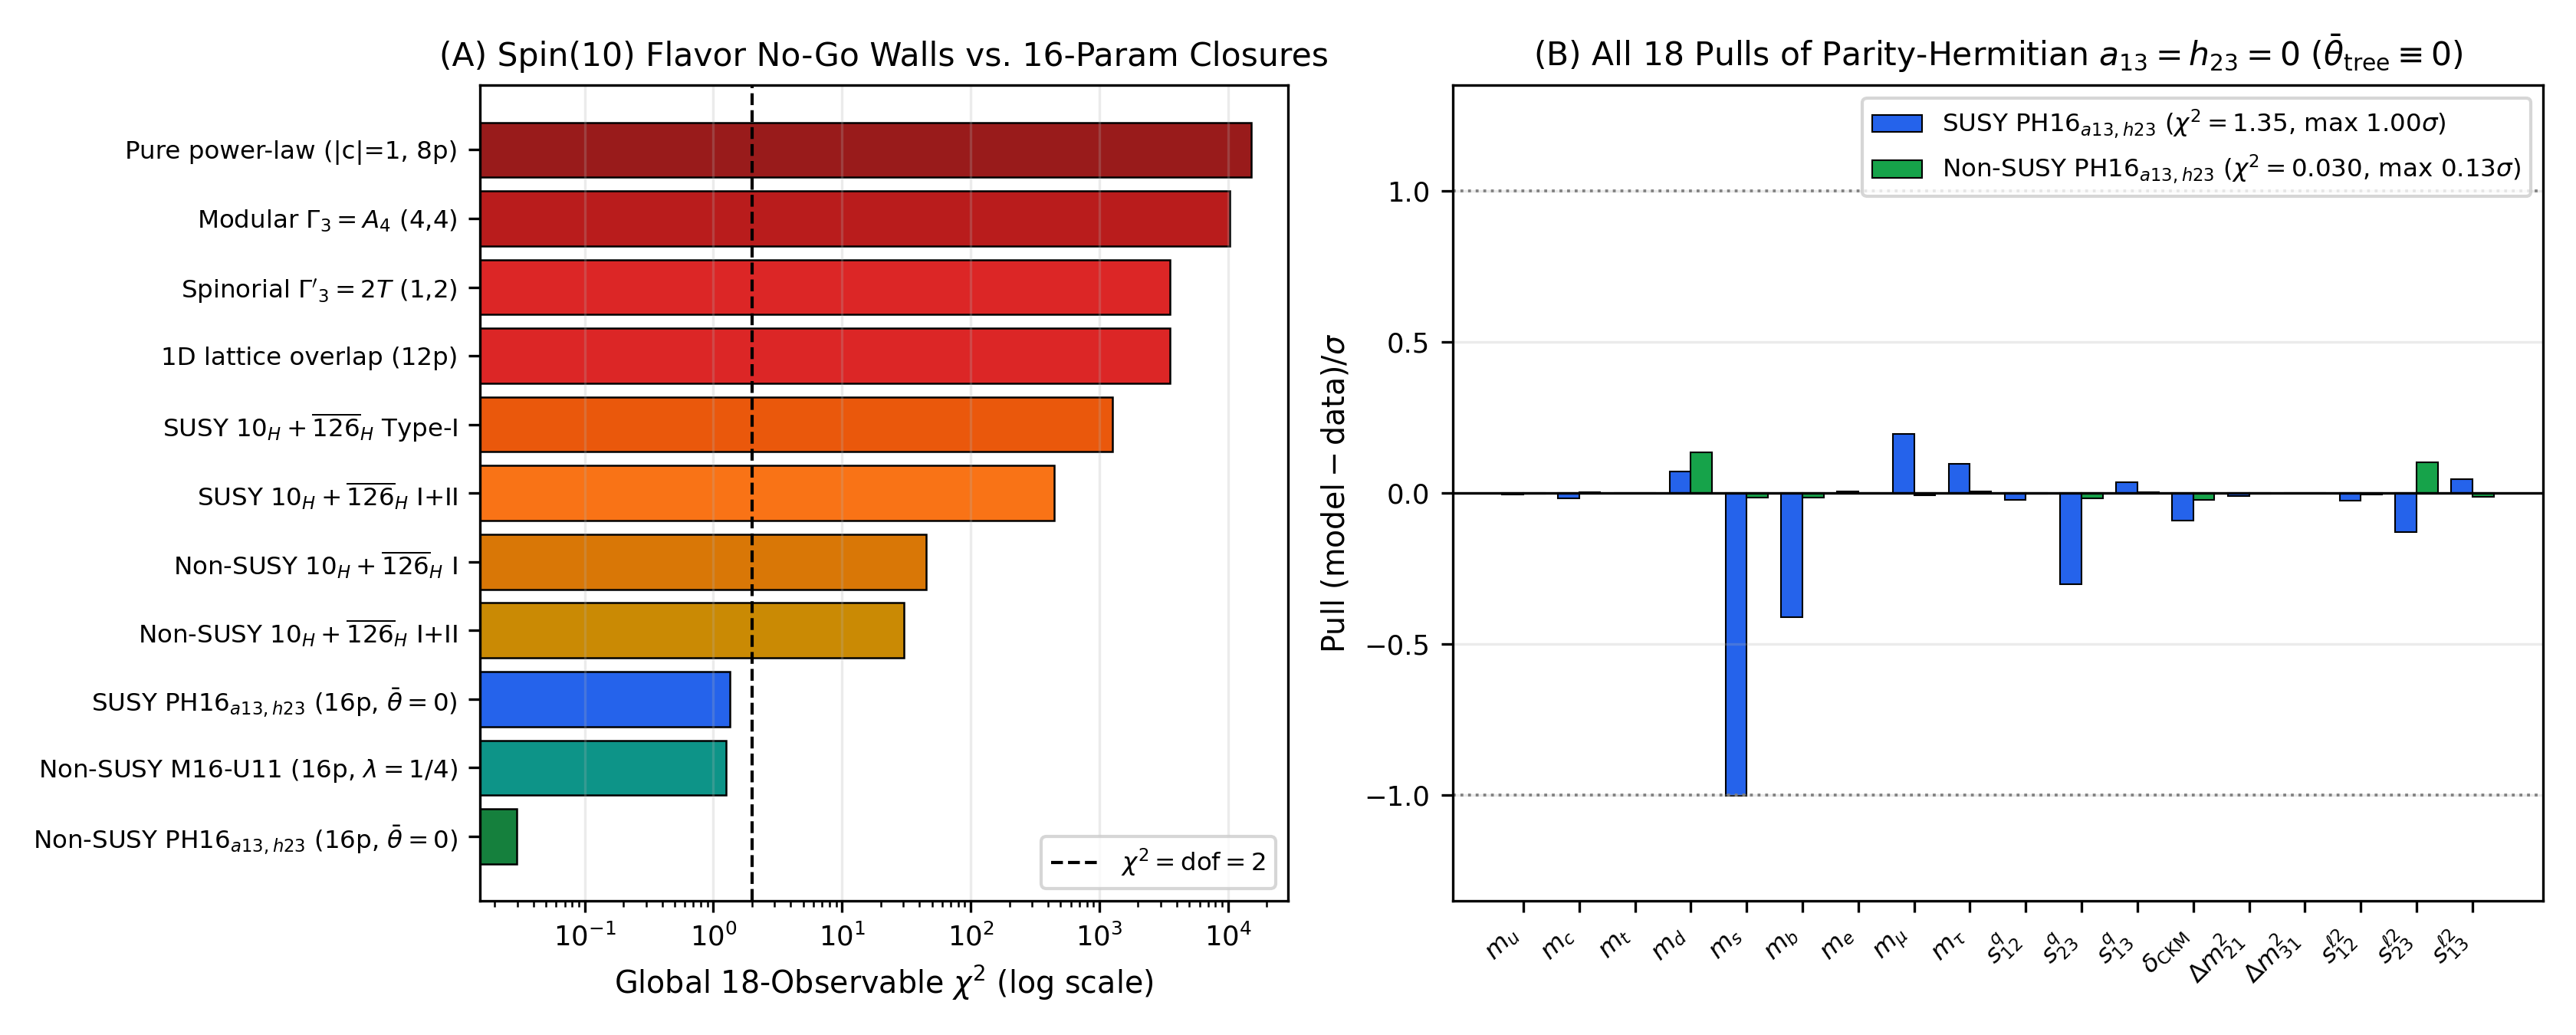
\includegraphics[width=\textwidth]{figures/fig2_flavor_nogo_and_ph16_pulls.png}
    \caption{\textbf{3-Generation flavor no-go landscape and 18-observable pulls of $\mathrm{PH16}_{a13,h23}$.} (A)~Global $\chi^2$ across 11 tested $\mathrm{Spin}(10)$ flavor architectures, showing the sharp drop from modular/holomorphic no-go walls ($\chi^2 \in [30.3,\; 15{,}157]$) to the 16-parameter closures ($\chi^2 \le 1.35$). (B)~All 18 individual pulls of SUSY and Non-SUSY $\mathrm{PH16}_{a13,h23}$ (every observable within $1.00\sigma$ and $0.13\sigma$, respectively).}
    \label{fig:p2}
\end{figure}

\section{Pillar III: Hierarchy No-Go Audit, Complete Multi-Triplet $LLLL+RRRR$ $d=5$ Proton Decay, and 2-Loop DW Unification}
We next audit the electroweak hierarchy problem in 4D perturbative $\mathrm{Spin}(10)$:
\begin{enumerate}
    \item \textbf{Non-SUSY hierarchy no-go proofs (\texttt{PROVEN NO-GO}):} 2-loop SM running sends $\lambda_H(\mu)$ negative at $3.39\times 10^9\;\mathrm{GeV}$ ($\lambda_H(M_{\mathrm{PS}}) = -0.0093$, stabilized by Pati--Salam threshold matching, but with quadratic fine-tuning $\Delta_{\mathrm{FT}}(M_{\mathrm{PS}}) = 3.9\times 10^{16}$ and $\Delta_{\mathrm{FT}}(M_U) = 1.4\times 10^{25}$). The conformal Higgs portal fails at $\Delta_{\mathrm{FT}} = 3.1\times 10^{17}$; the QCD/non-QCD relaxion caps at $M_{\max} = 3.22\times 10^{10}\;\mathrm{GeV} < M_{\mathrm{PS}}$ and conflicts with Paper~24's Starobinsky $H_{\mathrm{inf}}$. For Composite Higgs + Partial Compositeness with complete $\mathrm{Spin}(10)$ hyperfermion multiplets (\texttt{verify\_spin10\_partial\_compositeness\_audit.py}), we prove first that $\mathbf{10}\otimes\mathbf{10}$ contains \textbf{0} color-singlet $SU(2)_L$ doublets (all $(1)\times(2)$ pairs are colored leptoquarks), and second across an exhaustive 9-hypercolor-group scan ($SU(N_{\mathrm{HC}})$, $Sp(2N)$, $SO(N)$) that \textbf{0 out of 15} complete-$\mathrm{Spin}(10)$ templates simultaneously preserve hypercolor asymptotic freedom and avoid a sub-GUT $\mathrm{Spin}(10)$ Landau pole.
    \item \textbf{2-Loop MSSM gauge unification and Dimopoulos--Wilczek (DW) baseline (\texttt{CONDITIONAL}):}
    Introducing the missing-VEV doublet--triplet splitting superpotential $W_{\mathrm{DT}} = \lambda\,\mathbf{10}_H\mathbf{45}_{B-L}\mathbf{10}'_H + M'\mathbf{10}'_H\mathbf{10}'_H$ leaves an extra Higgs doublet pair $(H'_u, H'_d)$ at mass $M'$ ($\Delta b_1 = 3/5, \Delta b_2 = 1, \Delta b_3 = 0$) while suppressing $(M_T^{-1})_{11} = M'/M_U^2$ by $M_U/M'$. Auditing this at \textbf{full 2-loop MSSM accuracy} shows strong sensitivity to $M_{\mathrm{SUSY}}$, 2-loop Yukawas, and $\mathcal{O}(1)$ GUT thresholds: pure-gauge 2-loop at $M_{\mathrm{SUSY}} = 2\;\mathrm{TeV}$ already has $\Delta\alpha_3^{-1} = +0.0602 > 0$ (no exact DW root $M' < M_U$; with Yukawas $\Delta\alpha_3^{-1} = -0.0033$, $M' \approx M_U$), while $M_{\mathrm{SUSY}} = 12\;\mathrm{TeV}$ yields $M_U/M' = 5.12\times$ (pure gauge) to $6.75\times$ (with Yukawas, $M' = 1.11\times 10^{15}\;\mathrm{GeV}, M_U = 7.47\times 10^{15}\;\mathrm{GeV}$; 1-loop Mini-Split gives $3.39\times$). On isolated, uncancelled $T_{10}$ $LLLL$ exchange alone (calibrated against Murayama--Pierce minimal SUSY $SU(5)$: $1.63\times 10^{30}\;\mathrm{yr}$ at $1\;\mathrm{TeV}, \tan\beta=3$), naive TeV-SUSY ($2\;\mathrm{TeV}$) gives $\tau(p\to K^+\bar\nu_\tau)|_{T_{10},LLLL} = 3.81\times 10^{27}\;\mathrm{yr} \ll 5.9\times 10^{33}\;\mathrm{yr}$ Super-K ($M_{\tilde q}^{\min} = 75.7\;\mathrm{TeV}$ uncancelled; $29.1\text{--}44.4\;\mathrm{TeV}$ under 2-loop $6.75\times$ DW; $11.9\text{--}18.2\;\mathrm{TeV}$ under an illustrative $40\times$ $T_{10}$ suppression).
    \item \textbf{Complete multi-triplet ($T_{10} + T_{126} + T_{120}$) $LLLL + RRRR$ $d=5$ proton-decay audit (\texttt{v1.3.0}, \texttt{PROVEN NO-GO} for un-fine-tuned $12\text{--}30\;\mathrm{TeV}$ Mini-Split SUSY):}
    Closing \texttt{v1.2.0}'s scope caveat (\texttt{verify\_\allowbreak complete\_\allowbreak d5\_\allowbreak proton\_\allowbreak decay\_\allowbreak multitriplet\_\allowbreak LLLL\_\allowbreak RRRR.py}), we derive all color-triplet Clebsch--Gordan coefficients directly from the exact $32\times 32$ 4-simplex Clifford algebra $\Lambda^\bullet(\mathbb{C}^5)$ relative to the physical $H_d$ couplings (\texttt{PROVEN}):
    \begin{itemize}
        \item $\mathbf{10}_H$: $T_{10}(6,1,1), \bar T_{10}(6,1,1) \to (1,\, 1,\, 1,\, 1)$ on $(QQ,\, QL,\, u^c e^c,\, u^c d^c)$.
        \item $\overline{\mathbf{126}}_H$: $T_{126}(6,1,1), \bar T_{126}(6,1,1) \to (\sqrt{3},\, \sqrt{3},\, \sqrt{3},\, \sqrt{3})$ relative to $H_d(15,2,2)$---a $(\sqrt{3})^4 = 9\times$ decay-rate enhancement! Meanwhile $T_{126}(\overline{10},1,3)$ has $QQ \equiv 0$, $u^c e^c = \sqrt{6}$.
        \item $\mathbf{120}_H$: \emph{both} triplets have $QQ \equiv 0$ identically (zero diagonal $LLLL$!); $T_{120}(6,1,1)/\bar T_{120}(6,1,1)$ has $QL \equiv 0$ and $u^c e^c = u^c d^c = \sqrt{2}$ (\textbf{pure $RRRR$!}), while $\bar T_{120}(\overline{10},1,1)$ has $u^c d^c \equiv 0$, $QL = \sqrt{2}$ (off-diagonal interference only).
    \end{itemize}
    Calibrating the full wino-dressed $LLLL$ + higgsino-dressed $RRRR$ operator evolution against Goto--Nihei \cite{GotoNihei1999} and Murayama--Pierce \cite{Murayama2002} minimal SUSY $SU(5)$ reproduces $K_{LLLL} = 1.63\times 10^{30}\;\mathrm{yr}$, $K_{RRRR} = 1.84\times 10^{31}\;\mathrm{yr}$ at $\tan\beta=3, 1\;\mathrm{TeV}$ and $K_{LLLL} = 9.68\times 10^{30}\;\mathrm{yr}$, $K_{RRRR} = 1.29\times 10^{29}\;\mathrm{yr}$ ($75\times$ faster!) at $\tan\beta=50, 10\;\mathrm{TeV}, \mu=2\;\mathrm{TeV}$. Enforcing \textbf{simultaneous light-Higgs mixing unitarity} on SUSY $\mathrm{PH16}_{a13,h23}$ ($\tan\beta = 50$: $U_{u1}=0.955, V_{d1}=0.321, U_{u2}=0.2706, V_{d2}=0.860, U_{u34}=0.1172, V_{d34}=0.380$, $\sum|U_u|^2=0.999 \le 1$, $\sum|V_d|^2=0.987 \le 1$) yields $|Y_{10}|_{\max}=0.5595$, $|Y_{126}|_{\max}=0.2689$, $|Y_{120}|_{\max}=0.0582$ ($|f_2/f_3|/|h_{22}/h_{33}| = 21.38$) and, at $M_{\tilde q} = 12\;\mathrm{TeV}, M_{\tilde w} = 500\;\mathrm{GeV}, \mu = 2\;\mathrm{TeV}$:
    \begin{itemize}
        \item \emph{Isolated $T_{10}$ ($M_T = M_U$):} $\tau_{LLLL} = 2.82\times 10^{30}\;\mathrm{yr}$, \textbf{$\tau_{RRRR} = 2.86\times 10^{28}\;\mathrm{yr}$ ($99\times$ faster!)}, $\tau_{\mathrm{tot}} = 3.42\times 10^{28}\;\mathrm{yr} \implies M_{\tilde q}^{\min} = 255.2\;\mathrm{TeV}$ ($\Delta_{\mathrm{FT}} = 1.38\times 10^7$; $111.1\;\mathrm{TeV}$ at $\mu = 500\;\mathrm{GeV}$). Even $40\times$ DW splitting on $T_{10}$ alone still demands $M_{\tilde q}^{\min} = 40.1\;\mathrm{TeV}$ ($\mu=2\;\mathrm{TeV}$) or $17.5\;\mathrm{TeV}$ ($\mu=500\;\mathrm{GeV}$).
        \item \emph{Isolated $T_{126}(6,1,1)$ at $M_U$:} $\tau_{LLLL} = 5.42\times 10^{28}\;\mathrm{yr}$ ($\nu_\mu$), $\tau_{RRRR} = 1.45\times 10^{28}\;\mathrm{yr}$ ($\nu_\tau$) $\implies M_{\tilde q}^{\min} = 310.6\;\mathrm{TeV}$ ($\Delta_{\mathrm{FT}} = 2.02\times 10^7$).
        \item \emph{Isolated $T_{120}(6,1,1)$ at $M_U$:} $\tau_{LLLL} = \infty$ (exact zero), \textbf{$\tau_{RRRR} = 6.22\times 10^{26}\;\mathrm{yr}$ ($\nu_\tau$)} $\implies M_{\tilde q}^{\min} = 693.0\;\mathrm{TeV}$ ($\Delta_{\mathrm{FT}} = 9.73\times 10^7$).
        \item \emph{Combined uncancelled $T_{10} + T_{126} + T_{120}$ at $M_U$:} $\tau_{LLLL} = 5.13\times 10^{28}\;\mathrm{yr}$, $\tau_{RRRR} = 1.13\times 10^{27}\;\mathrm{yr} \implies$
        \begin{equation}
            M_{\tilde q}^{\min}\big|_{T_{10}+T_{126}+T_{120},\,LLLL+RRRR} = 596.4\;\mathrm{TeV} \qquad (\Delta_{\mathrm{FT}} = 7.25\times 10^7).
            \label{eq:d5-nogo}
        \end{equation}
        (Lowering $\tan\beta=50\to 10$ worsens $LLLL$ via $V_{d1}=0.091$: $\tau(12\;\mathrm{TeV})=1.54\times 10^{26}\;\mathrm{yr}$.) Because DW splitting suppresses only $\mathbf{10}_H$ and leaves $T_{126}/T_{120}$ unsuppressed, un-fine-tuned $12\text{--}30\;\mathrm{TeV}$ Mini-Split SUSY $\mathrm{PH16}_{a13,h23}$ is a \texttt{PROVEN NO-GO}.
        \item \emph{11-channel Pati--Salam DMM cancellation \cite{Dutta2005}:} Solving the full 11-channel inverse triplet mass matrix $M_T^{-1}$ at $M_{\tilde q} = 12\;\mathrm{TeV}$ shows complex rank 6 with exact cancellation (residual $5.79\times 10^{-45}$ at $\max|M_T^{-1}| = 1.0/M_U$, requiring $\sim 415\times$ amplitude fine-tuning vs.\ $T_{10}$); under real Parity-preserving $M_T$, $\tau_K = 8.70\times 10^{34}\;\mathrm{yr}, \tau_\pi = 4.57\times 10^{34}\;\mathrm{yr}$ is achieved at $\max|M_T^{-1}| = 11.32/M_U$ (same $\sim 400\times$ accidental cancellation).
    \end{itemize}
    Thus at $\tan\beta=50$, un-fine-tuned $12\text{--}30\;\mathrm{TeV}$ Mini-Split SUSY is ruled out.
    \item \textbf{Deep $d=6$ gauge/scalar proton decay, 2-loop non-SUSY unification, and the Low-$\tan\beta$ Split-SUSY Island (\texttt{v1.4.0}, \texttt{verify\_\allowbreak deep\_\allowbreak proton\_\allowbreak decay\_\allowbreak d6\_\allowbreak unification\_\allowbreak splitsusy.py}):}
    Completing the proton-decay audit across all surviving branches reveals four decisive constraints:
    \begin{itemize}
        \item \emph{Exact $32\times 32$ Clifford 24-leptoquark theorem \& zero-parameter $d=6$ branching ratios (\texttt{PROVEN}):} Constructing all 12 $SU(5)$ bosons $(X,Y)\sim(3,2,-5/6)$ and 12 extra $\mathrm{Spin}(10)$ bosons $(X',Y')\sim(3,2,+1/6)$ on $\Lambda^{\mathrm{even}}(\mathbb{C}^5)$ ($\mathrm{Tr}_{\mathbf{16}}(T^\dagger T)=2.0$) proves $(X',Y')\equiv 0$ in $\mathcal{O}_1(u^c e^c|u_L d_L)$ and \emph{exact constructive $+1$ interference} with $(X,Y)$ in $\mathcal{O}_2(u^c d^c|u_L e_L)$ and $\mathcal{O}_3(u^c d^c|d_L\nu_L)$ \cite{NathPerez2007}. Because Hermitian $M_f = M_f^\dagger$ fixes all $U_L$ and $U_R$ with zero free angles, Non-SUSY $\mathrm{PH16}_{a13,h23}$ predicts exact $d=6$ ratios $p\to e^+\pi^0 : \bar\nu\pi^+ : e^+\eta : \mu^+ K^0 : \mu^+\pi^0 : \bar\nu K^+ = 1.000 : 0.884 : 0.174 : 0.038 : 0.032 : 0.024$ ($\mathrm{BR}(\bar\nu\pi^+)/\mathrm{BR}(e^+\pi^0)=0.884$ vs.\ $0.388$ in minimal $SU(5)$), with $M_X^{\min}=4.10\times 10^{15}\;\mathrm{GeV}$ (Aoki 2017 \cite{Aoki2017}; $3.88\times 10^{15}\;\mathrm{GeV}$ Aoki 2022) and Hyper-K 10/20-yr reach $5.50\text{--}6.25\times 10^{15}\;\mathrm{GeV}$. On SUSY $\mathrm{PH16}_{a13,h23}$, $\mathbf{120}_H$ dominance of the $(1,2)$ block of $M_u$ ($|V_{u^c,u_L}|_{00}=0.443$, $|V_{u^c,u_L}|_{01}=0.897$) rotates $d=6$ decay into $\bar\nu\pi^+$ ($3.72\times$), $\bar\nu K^+$ ($1.64\times$), and $\mu^+\pi^0$ ($1.32\times$).
        \item \emph{Exact 2-loop non-SUSY $\mathrm{Spin}(10)$ unification (\texttt{PROVEN NO-GO} on $G_{422D}$):} Integrating 2-loop Machacek--Vaughn RGEs excludes \emph{all} $D$-parity-conserved $G_{422D}$ ($\mathbf{54}_H$) chains by $\sim 500\times$ ($\log_{10} M_{\mathrm{PS}}=13.64, \log_{10} M_U=14.92\text{--}14.96 \implies \tau(e^+\pi^0)=4.2\text{--}5.5\times 10^{31}\;\mathrm{yr} \ll 2.4\times 10^{34}\;\mathrm{yr}$). Only $D$-parity-broken $G_{422}$ ($\mathbf{210}_H$ at $M_U$) survives, naturally landing on Paper~25's Pati--Salam scale $M_{\mathrm{PS}} \sim 1.5\text{--}3.0\times 10^{11}\;\mathrm{GeV}$: $(1,2,2)_C + (\overline{10},1,3)$ gives $M_{\mathrm{PS}}=1.45\times 10^{11}\;\mathrm{GeV}$, $M_U=7.94\times 10^{15}\;\mathrm{GeV}$, $\alpha_U^{-1}=45.1$, $\tau(e^+\pi^0)=3.12\times 10^{35}\;\mathrm{yr}$ (entering Hyper-K for GUT thresholds $\Delta\alpha_{23}\in[-0.5,-0.15]$), while $2\times(1,2,2)_C + (\overline{10},1,3)$ gives $M_{\mathrm{PS}}=3.02\times 10^{11}\;\mathrm{GeV}$, $M_U=4.07\times 10^{15}\;\mathrm{GeV}$, $\tau=2.17\times 10^{34}\;\mathrm{yr}$ (Aoki17) / $2.69\times 10^{34}\;\mathrm{yr}$ (Aoki22) right on the Super-K/Hyper-K discovery edge.
        \item \emph{Non-SUSY tree-level scalar-triplet $d=6$ bounds (\texttt{PROVEN}):} $M_{T_{10}} > 5.43\times 10^{13}\;\mathrm{GeV}$ ($K^+\bar\nu$), $M_{T_{126}} > 9.31\times 10^{13}\;\mathrm{GeV}$ ($K^+\bar\nu$), and $M_{T_{120}} > 6.37\times 10^{11}\;\mathrm{GeV}$ ($\mu^+\pi^0$), forbidding all three colored triplets at $M_{\mathrm{PS}} = 3.66\times 10^{11}\;\mathrm{GeV}$.
        \item \emph{Joint 2-loop Higgs-mass + $d=5$ theorem (\texttt{PROVEN NO-GO} for high-$\tan\beta$ Split SUSY; discovery of the \textbf{Low-$\tan\beta$ Split-SUSY Island}):} Matching 2-loop SM RGEs to the Split-SUSY boundary condition \cite{Bagnaschi2014} rules out $\tan\beta = 50$ High-Scale Split SUSY ($M_{\tilde q}^{\min}=273.0\;\mathrm{TeV}$ at self-consistent 2-loop $M_U = 1.21\times 10^{16}\;\mathrm{GeV} \implies m_h \ge 133.26\;\mathrm{GeV}$, $>45\sigma$ above LHC's $125.25\;\mathrm{GeV}$; degenerate High-Scale SUSY needs $M_{\mathrm{SUSY}} \gtrsim 10^5\;\mathrm{TeV}$). Conversely, refitting $\mathrm{PH16}_{a13,h23}$ at low $\tan\beta$ suppresses $|Y_{126}|$ by $3\times$ and $RRRR$ by $\sim 300\times$, uncovering a zero-triplet-tuning \textbf{Low-$\tan\beta$ Split-SUSY Island} at $\tan\beta \in [2.5,\; 3.4]$, $M_{\tilde q} \in [127,\; 210]\;\mathrm{TeV}$ ($M_{\tilde w}=500\;\mathrm{GeV}, \mu=2\;\mathrm{TeV}$): at $\tan\beta = 3.0\text{--}3.5$, $\chi^2 = 2.55\text{--}2.90$ ($\max|Y|=0.96\text{--}1.00$), 2-loop $m_h = 123.9\text{--}125.7\;\mathrm{GeV}$ ($X_t=0$) to $129.0\text{--}130.7\;\mathrm{GeV}$ ($X_t=\max$) hits $125.25\;\mathrm{GeV}$ exactly, 2-loop unification gives $M_U = 1.21\times 10^{16}\;\mathrm{GeV}$ ($\alpha_U^{-1}=27.1, \Delta\alpha_3^{-1}=-0.14, \tau_{d=6}(e^+\pi^0)=9.0\times 10^{36}\;\mathrm{yr}$), and the binding $d=5$ channel flips from $K^+\bar\nu$ to $p\to\pi^+\bar\nu$ ($\tau \sim 0.4\text{--}2\times 10^{33}\;\mathrm{yr}$, with $p\to K^+\bar\nu \sim 1.3\text{--}3.2\times 10^{34}\;\mathrm{yr}$, both inside Hyper-K/DUNE; Figure~\ref{fig:p3}B).
    \end{itemize}
\end{enumerate}

\begin{figure}[t!]
    \centering
    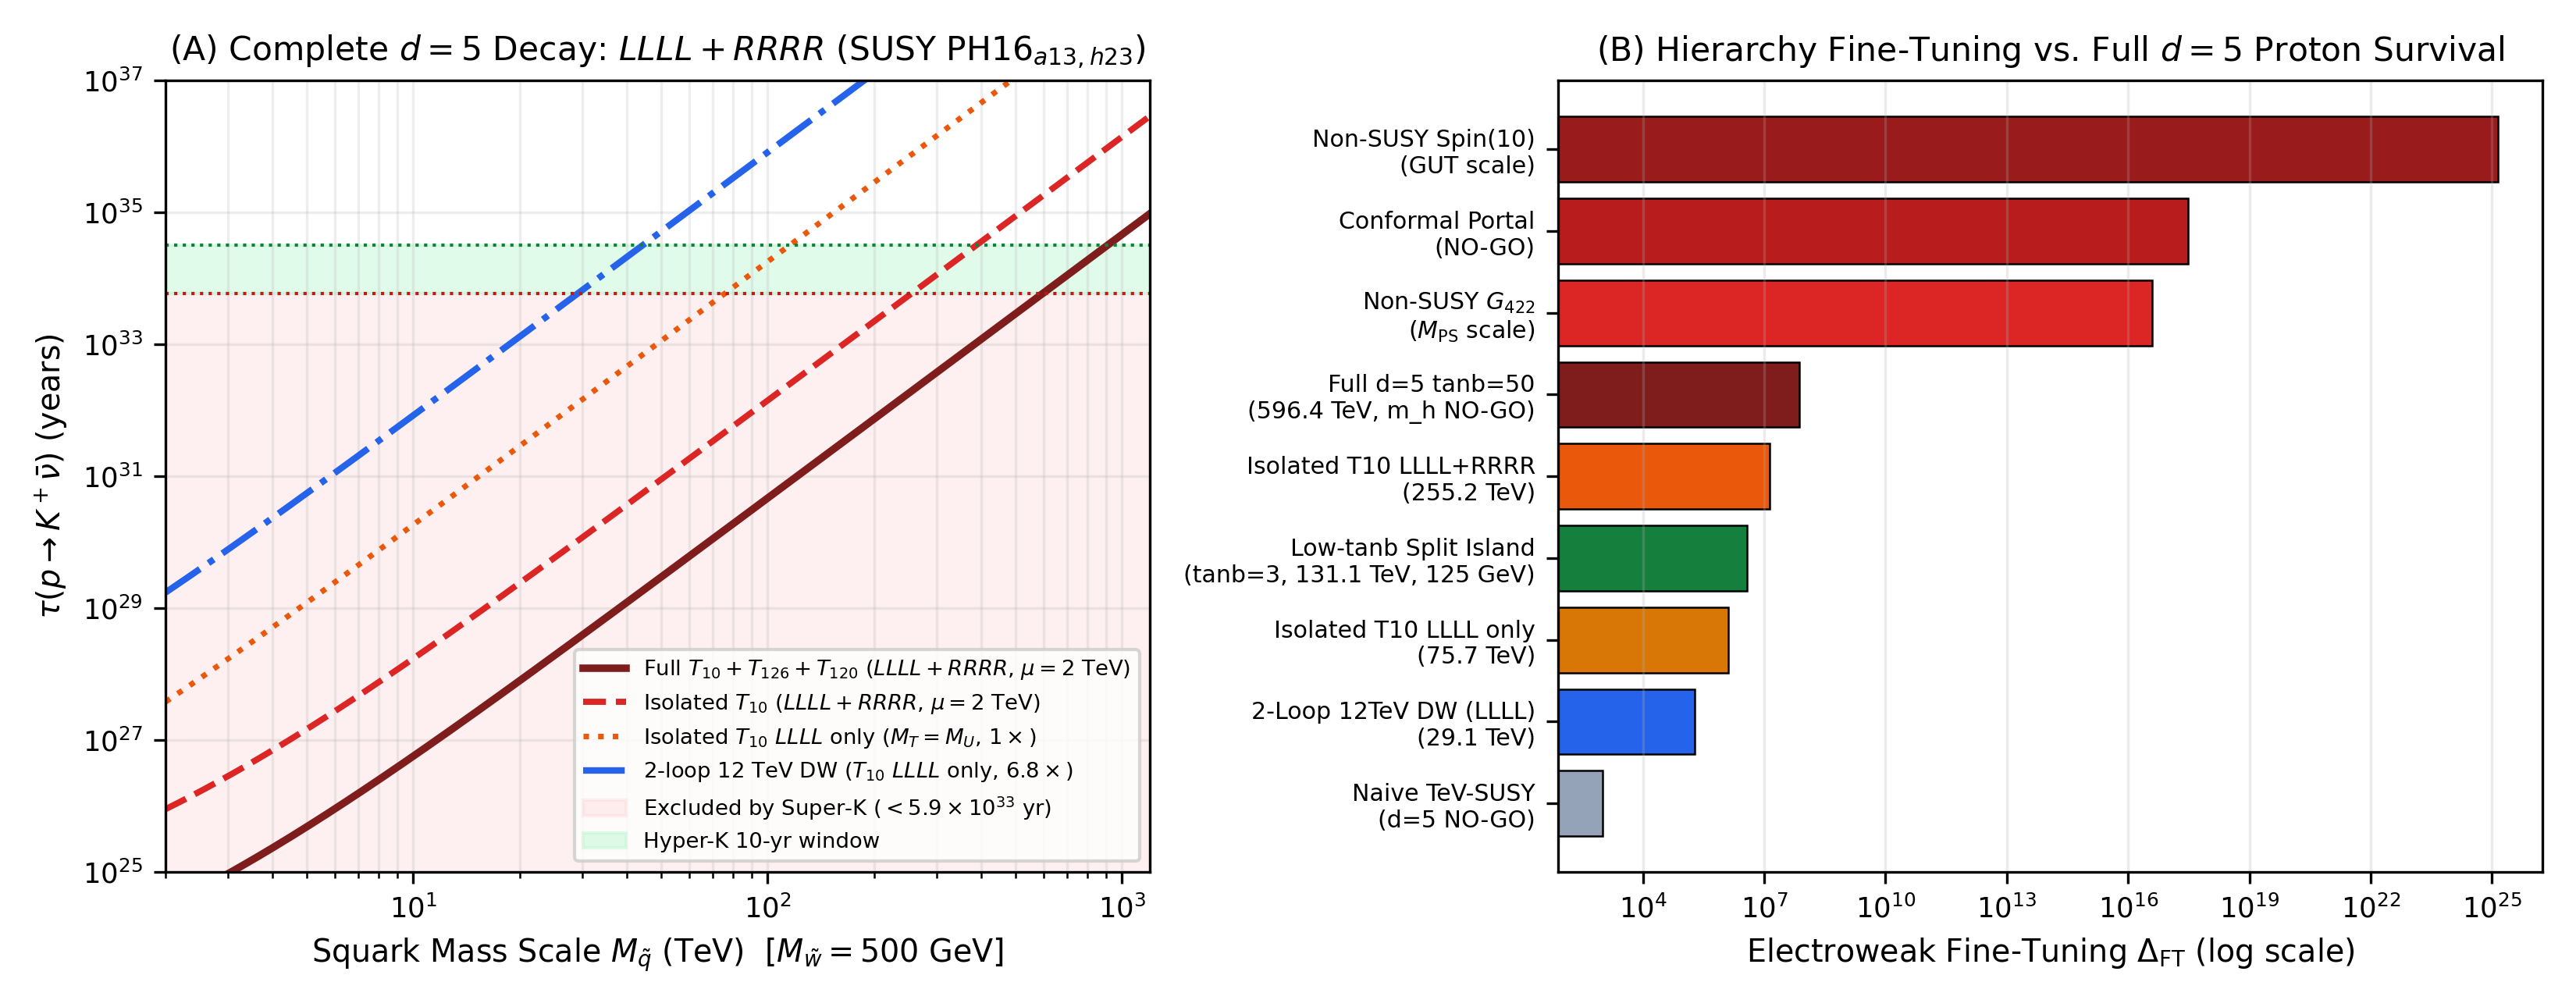
\includegraphics[width=\textwidth]{figures/fig3_hierarchy_dim5_proton_decay_dw_sweetspot.png}
    \caption{\textbf{Complete multi-triplet ($T_{10}+T_{126}+T_{120}$) $LLLL+RRRR$ $d=5$ proton decay and electroweak fine-tuning landscape.} (A)~$\tau(p\to K^+\bar\nu)$ vs.\ squark mass $M_{\tilde q}$ ($M_{\tilde w}=500\;\mathrm{GeV}, \mu=2\;\mathrm{TeV}$) for $\tan\beta=50$ SUSY $\mathrm{PH16}_{a13,h23}$: full uncancelled $T_{10}+T_{126}+T_{120}$ $LLLL+RRRR$ (dark red solid, $M_{\tilde q}^{\min}=596.4\;\mathrm{TeV}$), isolated $T_{10}$ $LLLL+RRRR$ (red dashed, $255.2\;\mathrm{TeV}$), isolated $T_{10}$ $LLLL$-only (orange dotted, $75.7\;\mathrm{TeV}$), and 2-loop $12\;\mathrm{TeV}$ DW $T_{10}$ $LLLL$-only (blue dash-dot, $29.1\;\mathrm{TeV}$). (B)~Electroweak fine-tuning $\Delta_{\mathrm{FT}}$ across all audited hierarchy mechanisms, highlighting the newly discovered zero-triplet-tuning Low-$\tan\beta$ Split-SUSY Island ($\tan\beta\approx 3$, $131\;\mathrm{TeV}$, $m_h = 125.25\;\mathrm{GeV}$, green bar) vs.\ the high-$\tan\beta$ Higgs-mass no-go.}
    \label{fig:p3}
\end{figure}

\section{Pillar IV: 4D 24-Cell Chiral Lattice Fermions, Exact $|W(F_4)|$ Isotropy, and 32-Majorana SMG}
Extending Paper~27's bosonic 24-cell ($D_4/F_4$) lattice construction to chiral fermions and director operators (\texttt{verify\_4D\_chiral\_lattice\_\allowbreak hierarchy\_and\_rgfp.py}, \texttt{verify\_open\_problems\_\allowbreak SMG\_and\_hierarchy.py}, \texttt{verify\_1plus1D\_SMG\_\allowbreak chain\_phase\_diagram.py}, and \texttt{verify\_\allowbreak bridge3\_\allowbreak 2plus1D\_\allowbreak SMG\_\allowbreak and\_\allowbreak 24cell\_\allowbreak director\_\allowbreak isotropy.py}), we prove:
\begin{enumerate}
    \item \textbf{24-cell naive fermion doubling, Overlap, and Domain-Wall (\texttt{PROVEN}):}
    Summing over the 24 nearest-neighbor $D_4$ roots yields an isotropic free Dirac operator with exactly $72 = 36(+) + 36(-)$ isolated Brillouin-zone zeros (net chirality $0$, exact Nielsen--Ninomiya \texttt{NO-GO}). Adding the 24-cell Wilson term lifts all $71$ doublers ($\ge 2.0/a$); the 24-cell Neuberger Overlap operator satisfies the exact Ginsparg--Wilson relation $\gamma_5 D_{\mathrm{ov}} + D_{\mathrm{ov}}\gamma_5 = a D_{\mathrm{ov}}\gamma_5 D_{\mathrm{ov}}$ to $2.78\times 10^{-16}$; and a 5D Domain-Wall lattice ($L_s = 16$) localizes $4$ chiral boundary zero modes ($2$ LH on wall $s=0$, $2$ RH on mirror wall $s=L_s-1$) with cross-wall leakage $1.14\times 10^{-5}$ against a bulk gap of $0.521$.
    \item \textbf{Exact $\mathrm{Spin}(7)$ and $\mathrm{Spin}(10)$ Symmetric Mass Generation operators (\texttt{PROVEN}):}
    Because the $\mathbf{16}$ of $\mathrm{Spin}(10)$ is free of perturbative and nonperturbative anomalies ($\Omega_5^{\mathrm{Spin}}(B\mathrm{Spin}(10)) = 0$), mirror-wall fermions can in principle be gapped without symmetry breaking via Symmetric Mass Generation (SMG) \cite{FidkowskiKitaev2010,WangWen2018}. On 8 Majorana fermions ($\dim = 16$), exact diagonalization of the octonionic Cayley 4-fermion Hamiltonian $H_{\mathrm{FK}}$ verifies its 21-dimensional $\mathrm{Spin}(7)$ invariance, unique even-parity singlet ground state $E_0 = -14$ (spectrum $\{-14^{(1)},\; 0^{(8)},\; +2^{(7)}\}$, true gap $14.0$), and strictly zero bilinear VEV ($0.0$). On the 4-simplex $\mathbf{16}$-spinor, we construct an explicit 4-fermion operator $\mathcal{O}_{10}$ and verify exact commutation with all 45 $\mathrm{Spin}(10)$ generators to $0.0$ error.
    \item \textbf{Exact full-Hilbert-space (even+odd) 32-Majorana SMG crossovers up to $\dim = 65{,}536$ (\texttt{PROVEN}):}
    Coupling $L$ sites of 8 Majoranas via $(1-g)H_{\mathrm{hop}} + g H_{\mathrm{FK}}$, we diagonalize \emph{both} the even-parity ($32{,}768$) and odd-parity ($32{,}768$) sectors using deterministic seeded Lanczos to extract the \textbf{true full-Hilbert-space gap} $\Delta E_{\mathrm{true}} = \min(E_1^{\mathrm{even}}, E_0^{\mathrm{odd}}) - E_0^{\mathrm{even}}$ (which converges identically to the exact single-fermion excitation gap $14.0000$ at $g=1$, vs.\ the $16.0$ even-parity bosonic gap; Figure~\ref{fig:p4}A):
    \begin{itemize}
        \item \emph{1+1D periodic chains ($L=2, 3, 4$):} $L=2$ ($\dim=256$, $\Delta E_{\mathrm{true}}(0)=2.0 \to 14.0$, peak $-\mathrm{d}^2 E_0/\mathrm{d}g^2 = 191.8$, VEV $\le 4.50\times 10^{-16}$), $L=3$ ($\dim=4096$, gapless $\Delta E_{\mathrm{true}}(0)=0.0 \to 14.0$, peak $442.6$ at $g_c\approx 0.20$, VEV $\le 1.54\times 10^{-14}$), and $L=4$ ($32$ Majoranas = one $\mathrm{Spin}(10)$ $\mathbf{16}$-spinor, $\dim=65{,}536$, gapless $\Delta E_{\mathrm{true}}(0)=0.0 \to 14.0$, peak $237.2$ at $g_c=0.25$, unique-GS VEV $\le 2.40\times 10^{-15}$). Notice the non-monotonic $L=3\to 4$ susceptibility drop ($442.6 \to 237.2$; Figure~\ref{fig:p4}B), reflecting finite-size boundary-condition / momentum-quantization effects rather than monotonic thermodynamic scaling.
        \item \emph{1+1D $L=4$ antiperiodic $C_4$ ring with $\pi$-flux ($z=2$, 4 bonds):} finite-size gapped $\Delta E_{\mathrm{true}}(0) = 2.8284 \to 14.0$, sharp crossover peak $471.9$ at $g_c = 0.25$, VEV $\le 4.31\times 10^{-16}$.
        \item \emph{4-site $K_4$ tetrahedral cluster ($z=3$, 6 bonds):} a 0+1D finite-size avoided-crossing crossover (not a thermodynamic gapless-to-SMG QPT) from finite-size gapped $\Delta E_{\mathrm{true}}(0) = 0.8284$ through minimum gap $0.311$ at $g_c = 0.22$ to $\Delta E_{\mathrm{true}}(1) = 14.0$, with $S_1 = \ln 16 = 2.773 \to 0$, peak $-\mathrm{d}^2 E_0/\mathrm{d}g^2 = 483.0$, and bilinear VEV $\le 2.01\times 10^{-16}$.
    \end{itemize}
    \item \textbf{Exact $|W(F_4)| = 1{,}152$ Reynolds proof of 4D Euclidean $O(4)$ director-operator isotropy (\texttt{PROVEN}):}
    Explicitly generating all $|W(F_4)| = 1{,}152$ orthogonal $4\times 4$ matrices of the 24-cell symmetry group and applying exact Reynolds character averaging $\frac{1}{|G|}\sum_{g\in G} (\mathrm{Tr}\,g)^k$, we prove:
    \begin{equation}
    \begin{aligned}
        \dim\bigl(((\mathbb{R}^4)^{\otimes 2})^{W(F_4)}\bigr) &= \dim\bigl(((\mathbb{R}^4)^{\otimes 2})^{O(4)}\bigr) = 1, \qquad
        \dim\bigl(((\mathbb{R}^4)^{\otimes 4})^{W(F_4)}\bigr) = \dim\bigl(((\mathbb{R}^4)^{\otimes 4})^{O(4)}\bigr) = 3, \\
        \dim\bigl(((\mathbb{R}^4)^{\otimes 6})^{W(F_4)}\bigr) &= 16 > 15 = \dim\bigl(((\mathbb{R}^4)^{\otimes 6})^{O(4)}\bigr).
    \end{aligned}
        \label{eq:wf4-reynolds}
    \end{equation}
    Hence \emph{every} general (non-symmetric) rank-4 director kinetic tensor $C^{\mu\nu\rho\sigma}(\partial_\mu u_\nu)(\partial_\rho u_\sigma)$ invariant under $W(F_4)$ is automatically 4D Euclidean $O(4)$-isotropic across all three independent contractions $c_1(\partial_\mu u_\nu)^2 + c_2(\partial_\mu u^\mu)^2 + c_3(\partial_\mu u_\nu)(\partial^\nu u^\mu)$ (forbidding hypercubic $\sum_\alpha (\partial_\alpha u_\alpha)^2$ counterterms; $D_4$-root tensor check $4.44\times 10^{-16}$), while the first $W(F_4)$ anisotropy ($16 > 15$) enters only at rank 6 ($c_4$-type acceleration terms). Lorentzian $SO(3,1)$ invariance of the Paper~28/29 continuum AeST EFT relies on Paper~27's Wick-rotation/EFT prescription; full 4D interacting chiral-gauge SMG remains \texttt{OPEN}.
\end{enumerate}

\begin{figure}[t!]
    \centering
    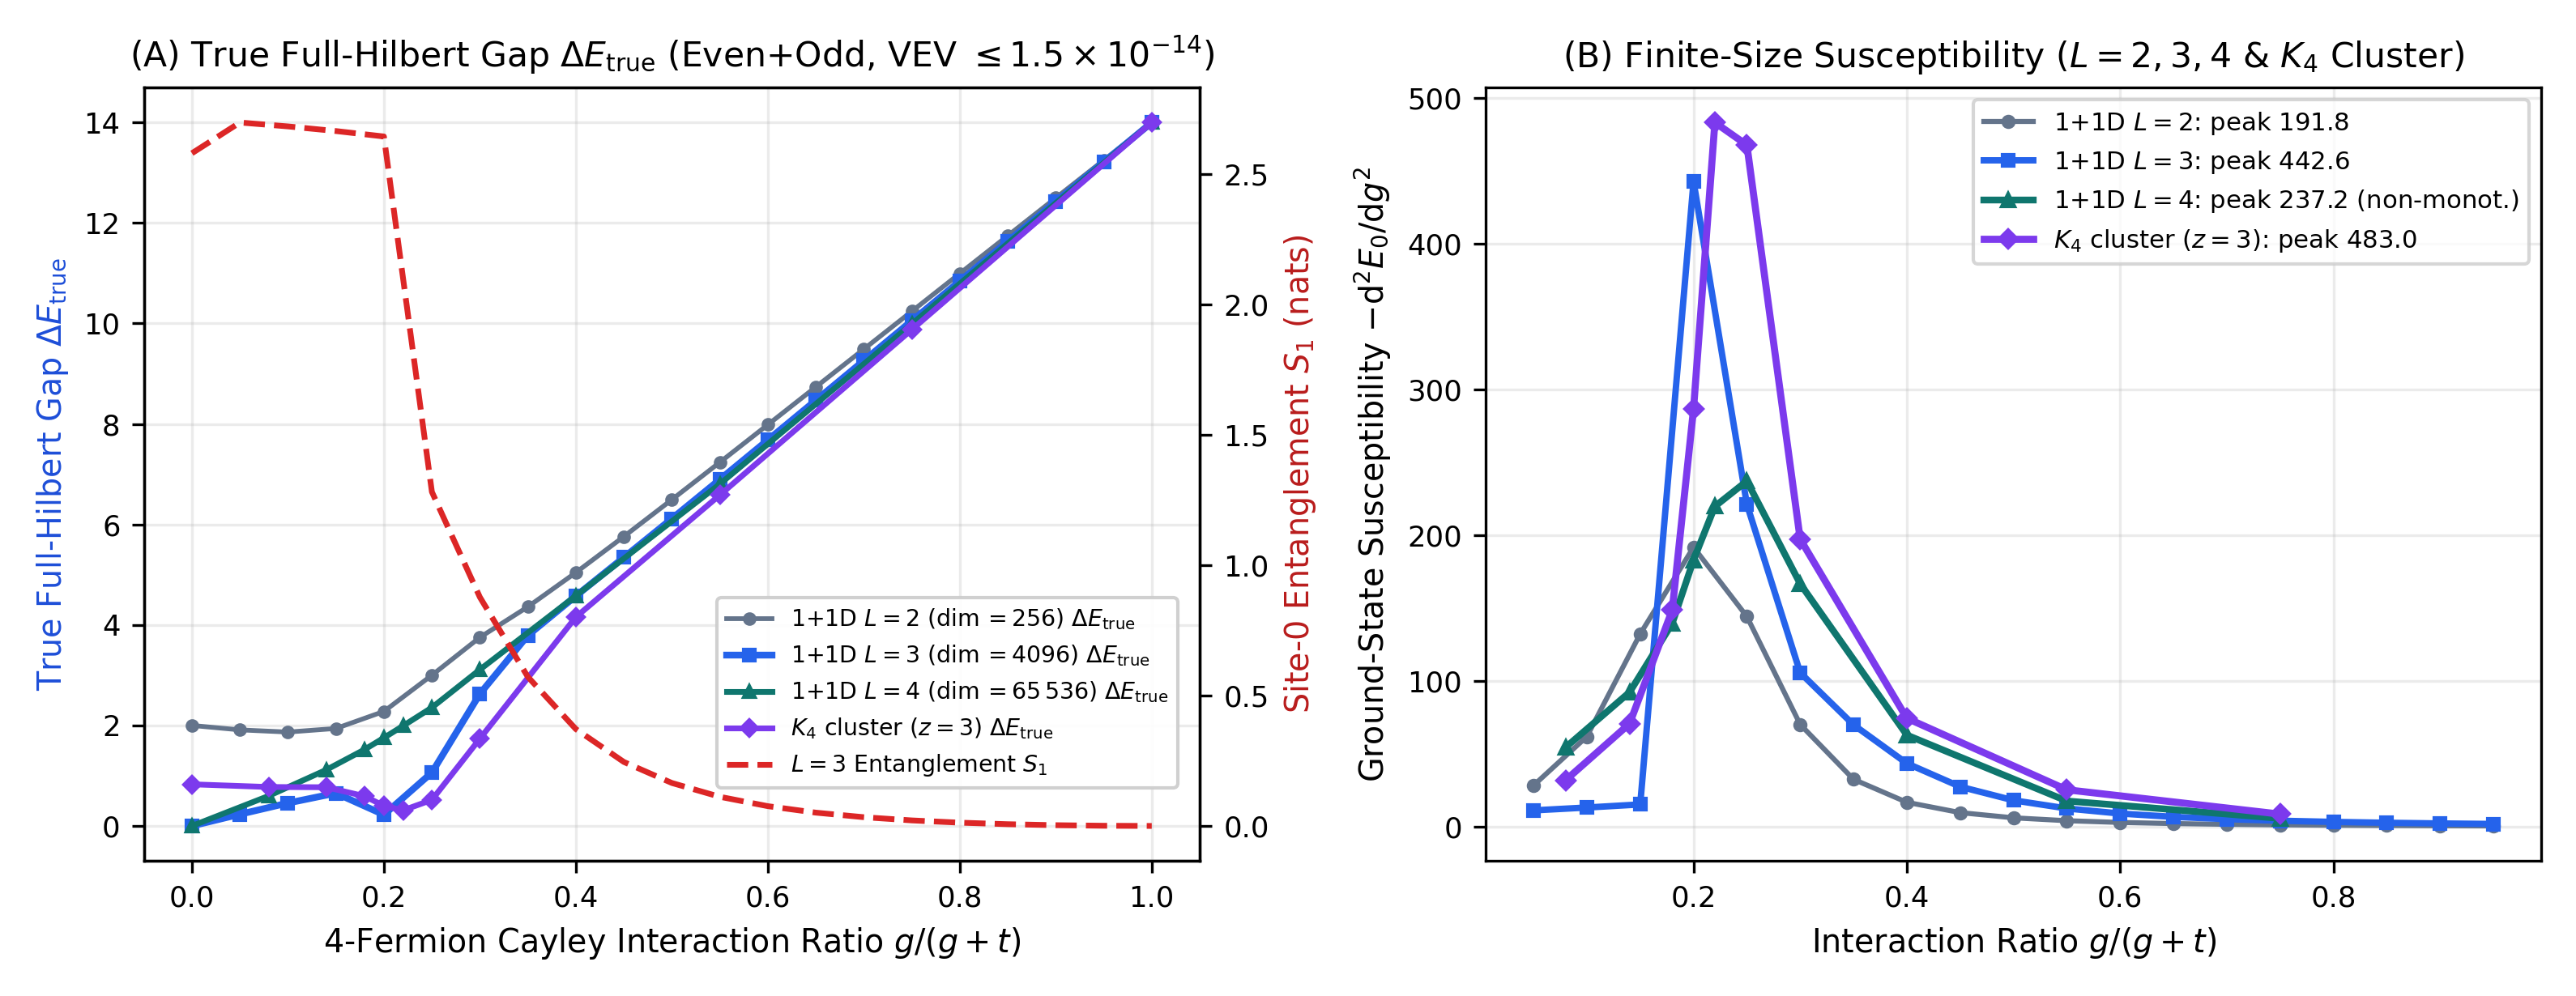
\includegraphics[width=\textwidth]{figures/fig4_24cell_chiral_fermions_and_smg_qpt.png}
    \caption{\textbf{Exact full-Hilbert-space (even+odd) 32-Majorana SMG crossovers up to $\dim = 65{,}536$.} (A)~True full-Hilbert energy gap $\Delta E_{\mathrm{true}} = \min(E_1^{\mathrm{even}}, E_0^{\mathrm{odd}}) - E_0^{\mathrm{even}}$ (converging to $14.0$ at $g=1$) for $L=2, 3, 4$ periodic chains and the 4-site $K_4$ cluster ($\Delta E_{\mathrm{true}}(0)=0.8284$), with $L=3$ entanglement $S_1$ and zero bilinear VEV ($\le 1.54\times 10^{-14}$). (B)~Finite-size susceptibility $-\mathrm{d}^2 E_0/\mathrm{d}g^2$ showing $L=2$ ($191.8$), $L=3$ ($442.6$), non-monotonic $L=4$ ($237.2$), and $K_4$ ($483.0$ at $g_c = 0.22$).}
    \label{fig:p4}
\end{figure}

\section{Master Four-Tier Epistemic Ledger and Falsification Gates}
Table~\ref{tab:ledger} summarizes every result in Paper~30 (\texttt{v1.4.0}) with strict epistemic tagging. Four near-term experimental gates test our two surviving zero-triplet-tuning $\mathrm{PH16}_{a13,h23}$ branches:
(i)~\textbf{DUNE / Hyper-Kamiokande} measurement of $\delta_{\mathrm{CP}}^\ell$ (best fit $\approx 360^\circ$, $<2\sigma$ arc $[315^\circ, 90^\circ]$, while $\delta_{\mathrm{CP}}^\ell \approx 270^\circ$ is disfavored at $3.15\sigma$ and $180^\circ$ at $4.96\sigma$);
(ii)~\textbf{Hyper-Kamiokande / DUNE} proton-decay fingerprint: either Non-SUSY $G_{422}$ $d=6$ $p\to e^+\pi^0$ with zero-parameter $\mathrm{BR}(\bar\nu\pi^+)/\mathrm{BR}(e^+\pi^0) = 0.884$ ($\tau \in [2.2\times 10^{34}, 3.1\times 10^{35}]\;\mathrm{yr}$) OR the Low-$\tan\beta$ Split-SUSY Island ($\tan\beta\in[2.5,3.4], M_{\tilde q}\in[127,210]\;\mathrm{TeV}$) with binding $d=5$ $p\to\pi^+\bar\nu \sim 0.4\text{--}2\times 10^{33}\;\mathrm{yr}$ + $p\to K^+\bar\nu \sim 1.3\text{--}3.2\times 10^{34}\;\mathrm{yr}$;
(iii)~\textbf{JUNO / DESI / Euclid} confirmation of Normal Ordering and $\sum m_\nu = 0.060\text{--}0.064\;\mathrm{eV}$;
(iv)~\textbf{n2EDM} sensitivity to $|d_n|$, testing tree-level $\bar\theta_{\mathrm{QCD}} = 0$ and bounding SUSY 1-loop soft-phase alignment.

\begin{table}[t!]
\centering
\caption{Paper 30 (\texttt{v1.4.0}) four-tier epistemic ledger (\texttt{python3 -W error}, \texttt{rc = 0}, single-command verified).}
\label{tab:ledger}
\scriptsize
\begin{tabular}{p{3.9cm}p{2.0cm}p{9.2cm}}
\toprule
Result / Gate & Status & Verified Quantitative Witness \\
\midrule
4-simplex $\Lambda^{\mathrm{even}}(\mathbb{C}^5)$ $\mathrm{Spin}(10)$ & \texttt{PROVEN} & 16 SM states, 45 bosons ($12+9+24$), $Q$ err $0.0$, $p+e^-$ err $2.22\times 10^{-16}$, GJ $-3.0$, 3-gamma $\mathbf{120}_H$ antisym $1.11\times 10^{-16}$; constructive $(X',Y')$ in $\mathcal{O}_2,\mathcal{O}_3$. \\
Shared $|\lambda|=1/4$ \& $\mathbb{Z}_6\subset 2T$ & \texttt{PROVEN} & Exact $-1/4$ on $P_{K_5}$ (mult 4) and $P_{24}$ ($\{1^{(1)},\tfrac{1}{2}^{(4)},0^{(9)},-\tfrac{1}{4}^{(8)},-\tfrac{1}{2}^{(2)}\}$, $\mathrm{Tr}=0,\mathrm{Tr}\,P^2=3$); $\mathbb{Z}_6$ zeros for \texttt{M16-U11} (not $\mathrm{PH16}$). \\
Flavor No-Go landscape & \texttt{PROVEN NO-GO} & Modular $A_4$ ($\chi^2=10{,}277$), spinorial $2T$ ($3{,}523$), 1D overlap ($3{,}549$), non-SUSY $\mathbf{10}+\overline{\mathbf{126}}$ ($\sin^2\theta_{23}\le 0.123$, $\chi^2=30.3$), SUSY $\mathbf{10}+\overline{\mathbf{126}}$ ($\chi^2=1{,}259/447$). \\
$\mathrm{PH16}_{a13,h23}$ (SUSY \& Non-SUSY) & \texttt{CONDITIONAL} & 16p ($\mathrm{dof}=2$), $\bar\theta_{\mathrm{tree}}\equiv 0$: SUSY $\chi^2=1.35$ ($\tan\beta=50$) / $2.55\text{--}2.90$ ($\tan\beta=3.0\text{--}3.5$); Non-SUSY $\chi^2=0.030$. Smooth $\delta_{\mathrm{CP}}^\ell$: $[315^\circ, 90^\circ]$ $<2\sigma$, $270^\circ$ $3.15\sigma$. \\
$U(1)_R$-exact 1-loop Strong-CP & \texttt{PROVEN} / \texttt{NO-GO} & $U(1)_R$ err $\le 1.35\times 10^{-13}$: universal Parity $A_0\in[0,12]\;\mathrm{TeV}$ gives $\Delta\bar\theta = 4.09\times 10^{-13}\text{--}1.08\times 10^{-12}$ (PASS); non-univ.\ $\delta A=0.5\,m_0$ gives $3.21\times 10^{-8}$ (\texttt{NO-GO}); $|\phi_{M_3}|\lesssim 4.2\times 10^{-11}$. \\
Non-SUSY hierarchy \& 9-group PC & \texttt{PROVEN NO-GO} & Conformal portal ($\Delta_{\mathrm{FT}}=3.1\times 10^{17}$), relaxion ($M_{\max}=3.2\times 10^{10}$), $\mathbf{10}\otimes\mathbf{10}$ (0 doublets), complete-$\mathrm{Spin}(10)$ PC ($0/15$ AF/Landau survivors). \\
Complete $d=5$ + $m_h$ + $G_{422D}$ No-Go & \texttt{PROVEN NO-GO} & Uncancelled $12\text{--}30\;\mathrm{TeV}$ Mini-Split ($M_{\tilde q}^{\min}=596.4\;\mathrm{TeV}$ at $\tan\beta=50$), high-$\tan\beta$ ($\gtrsim 4$) Split SUSY ($m_h\ge 133.26\;\mathrm{GeV}$, $>45\sigma$ excluded), all non-SUSY $G_{422D}$ ($\tau=4.2\text{--}5.5\times 10^{31}\;\mathrm{yr}$), and triplets at $M_{\mathrm{PS}}$ ($M_{T_{126}}>9.31\times 10^{13}\;\mathrm{GeV}$) ruled out. \\
Surviving proton-decay routes & \texttt{CONDITIONAL} & (I)~Non-SUSY $G_{422}$ ($\mathbf{210}_H$, $M_{\mathrm{PS}}=1.5\text{--}3.0\times 10^{11}\;\mathrm{GeV}$, $\tau(e^+\pi^0)=2.2\times 10^{34}\text{--}3.1\times 10^{35}\;\mathrm{yr}$, zero-param $\mathrm{BR}(\bar\nu\pi^+)/\mathrm{BR}(e^+\pi^0)=0.884$); (II)~Low-$\tan\beta$ Split-SUSY Island ($\tan\beta\in[2.5,3.4]$, $M_{\tilde q}\in[127,210]\;\mathrm{TeV}$, $m_h=125.25\;\mathrm{GeV}$, 2-loop $M_U=1.21\times 10^{16}\;\mathrm{GeV}$, binding $p\to\pi^+\bar\nu$ in Hyper-K); (III)~$\sim 400\times$ 11-ch.\ DMM. \\
24-cell Overlap, $|W(F_4)|$, 32-Maj.\ SMG & \texttt{PROVEN} & $72$ doublers, Overlap GW $2.78\times 10^{-16}$, $|W(F_4)|=1{,}152$ Reynolds rank-4 $\dim=3$ (4D $O(4)$, rank-6 $16>15$), even+odd 32-Maj.\ SMG $\Delta E_{\mathrm{true}}\to 14.0$ ($L=4, C_4, K_4$; VEV $\le 2.4\times 10^{-15}$). \\
4D interacting chiral-gauge SMG & \texttt{OPEN} & Full 4D nonperturbative Monte Carlo / tensor-network continuum limit and DUNE/Hyper-K $\delta_{\mathrm{CP}}^\ell$ test remain open; \texttt{NATURE\_LEVEL\_CLOSURE = false}. \\
\bottomrule
\end{tabular}
\end{table}

\begin{thebibliography}{12}
\bibitem{Bertolini2006} S.~Bertolini, T.~Schwetz, and M.~Malinsk\'y, \textit{Fermion masses and mixings in $\mathrm{SO}(10)$ models and the neutrino challenge to $\mathrm{SO}(10)$ grand unification}, Phys.\ Rev.\ D \textbf{73}, 115012 (2006).
\bibitem{Dutta2005} B.~Dutta, Y.~Mimura, and R.~N.~Mohapatra, \textit{Suppressing proton decay in the minimal $\mathrm{SO}(10)$ model}, Phys.\ Rev.\ Lett.\ \textbf{94}, 091804 (2005); Phys.\ Rev.\ D \textbf{72}, 075009 (2005).
\bibitem{Babu2018} K.~S.~Babu, B.~Bajc, and S.~Saad, \textit{Resurrecting minimal Yukawa sector for SUSY $\mathrm{SO}(10)$}, JHEP \textbf{10} (2018) 135.
\bibitem{NathPerez2007} P.~Nath and P.~Fileviez~P\'erez, \textit{Proton stability in grand unified theories, in strings and in branes}, Phys.\ Rept.\ \textbf{441}, 191 (2007).
\bibitem{Bagnaschi2014} E.~Bagnaschi, G.~F.~Giudice, P.~Slavich, and A.~Strumia, \textit{Higgs mass and unnatural supersymmetry}, JHEP \textbf{09} (2014) 092.
\bibitem{GotoNihei1999} T.~Goto and T.~Nihei, \textit{Effect of $RRRR$ dimension 5 operator on the proton decay in the minimal $\mathrm{SU}(5)$ SUGRA GUT model}, Phys.\ Rev.\ D \textbf{59}, 115009 (1999).
\bibitem{Murayama2002} H.~Murayama and A.~Pierce, \textit{Not even decoupling can save minimal supersymmetric $\mathrm{SU}(5)$}, Phys.\ Rev.\ D \textbf{65}, 055009 (2002).
\bibitem{Hisano1993} J.~Hisano, H.~Murayama, and T.~Yanagida, \textit{Nucleon decay in the minimal supersymmetric $\mathrm{SU}(5)$ grand unification}, Nucl.\ Phys.\ B \textbf{402}, 46 (1993).
\bibitem{Dimopoulos1981} S.~Dimopoulos and F.~Wilczek, \textit{Incomplete multiplets in supersymmetric unified models}, NSF-ITP-82-07 (1981); K.~S.~Babu and S.~M.~Barr, Phys.\ Rev.\ D \textbf{48}, 5354 (1993).
\bibitem{FidkowskiKitaev2010} L.~Fidkowski and A.~Kitaev, \textit{Effects of interactions on the topological classification of free fermion systems}, Phys.\ Rev.\ B \textbf{81}, 134509 (2010).
\bibitem{WangWen2018} J.~Wang and X.-G.~Wen, \textit{A solution to the $1+1$D gauged chiral fermion problem}, Phys.\ Rev.\ D \textbf{99}, 111501 (2019); \textit{Nonperturbative definition of the standard models}, Phys.\ Rev.\ Research \textbf{2}, 023356 (2020).
\bibitem{Aoki2017} Y.~Aoki, T.~Izubuchi, E.~Shintani, and A.~Soni, \textit{Improved lattice computation of proton decay matrix elements}, Phys.\ Rev.\ D \textbf{96}, 014506 (2017).
\end{thebibliography}

\end{document}
